%! Licence = CC BY-NC-SA 4.0

%! Author = mariuszindel
%! Date = 24. Jan 2021
%! Project = latex-test-template


%import template
%! Licence = CC BY-NC-SA 4.0

%! Author = mariuszindel
%! Date = 24. Jan 2021
%! Project = latex-test-template

\documentclass[a4paper, landscape, fontsize=10pt]{scrartcl} %-scrartcl = deutsche Sprache

% charset
\usepackage[T1]{fontenc}
\usepackage[utf8]{inputenc} %-inputenc = Umlaute möglich
\usepackage{ulem}

% use language german
\usepackage[ngerman]{babel} % with n is new spelling

% format page size
\usepackage{geometry}
\geometry{top=0.25cm,left=0.25cm,right=0.25cm,bottom=0.25cm}
%\textheight = 558pt

% tabular
\usepackage{tabularx}

% math
\usepackage{amsmath}
\usepackage{amssymb}
\usepackage{amsfonts}
\usepackage{enumitem}

% graphic
\usepackage{graphicx}
\graphicspath{{media/}}

% colors
\usepackage[dvipsnames]{xcolor}

% multi columns
\usepackage{multicol}

% make items compact
\setlist{topsep=0pt, leftmargin=3mm, nolistsep}
\setlength{\parindent}{0cm} % disable indention of text

% author and institute
\newcommand{\AUTHOR}{Marius Zindel }
\newcommand{\INSTITUTE}{Hochschule für Technik Rapperswil}

% define header and footer
\usepackage{fancyhdr}
\pagestyle{fancy}

%\fancyhead[RO]{\AUTHOR| \INSTITUTE}
%\fancyhead[LO]{\TITLE}
%\fancyfoot[RO]{\DELIVERYDATE}
%\fancyfoot[LO]{Created with \LaTeX}
\renewcommand\headrulewidth{0pt}
\renewcommand\footrulewidth{0pt}
%\headsep = -2pt
\footskip = 0pt

% define color
\definecolor{sectionColor}{HTML}{228B22}
\definecolor{subSectionColor}{HTML}{CB4154}
\definecolor{subSubSectionColor}{HTML}{FFFF00}
\definecolor{inlineCodeColor}{HTML}{FF00FF}
\definecolor{codeBackground}{RGB}{245,245,245}
\definecolor{gray}{rgb}{0.5,0.5,0.5}
\definecolor{darkGreen}{RGB}{0,150,0}
\definecolor{DarkPurple}{rgb}{0.4, 0.1, 0.4}

% define section format
\usepackage{sectsty}
\usepackage{titlesec}

\titleformat{name=\section}[block]{\sffamily\small}{}{0pt}{\colorsection}
\titlespacing*{\section}{0pt}{0pt}{0pt}
\newcommand{\colorsection}[1]{%
    \colorbox{sectionColor!40}{\parbox{0.98\linewidth}{\color{black}\thesection\ #1 }}} % 0.235\textwidth

% define subsection format
\titleformat{name=\subsection}[block]{\sffamily\small}{}{0pt}{\colorsubsection}
\titlespacing*{\subsection}{0pt}{0pt}{0pt}
\newcommand{\colorsubsection}[1]{%
    \colorbox{subSectionColor!40}{\parbox{0.98\linewidth}{\color{black}\thesubsection\ #1 }}}

% define subsubsection format
\titleformat{name=\subsubsection}[block]{\sffamily\small}{}{0pt}{\colorsubsubsection}
\titlespacing*{\subsubsection}{0pt}{0pt}{0pt}
\newcommand{\colorsubsubsection}[1]{%
    \colorbox{subSubSectionColor!50}{\parbox{0.98\linewidth}{\color{black}\thesubsubsection\ #1 }}}

% import code listings
\usepackage{listings}
\usepackage{beramono}
\input{./style/listings.tex}
\lstset{style=htmlcssjs}
\lstset{aboveskip=0pt, belowskip=0pt}
\lstset{basicstyle={\footnotesize\ttfamily}}
\lstset{
    literate=  % Allow for German characters in lstlistings.
        {Ö}{{\"O}}1
        {Ä}{{\"A}}1
        {Ü}{{\"U}}1
        {ü}{{\"u}}1
        {ä}{{\"a}}1
        {ö}{{\"o}}1
}

% dotted rule
\usepackage{dashrule}
\usepackage{tikz}
\usetikzlibrary{decorations.markings}
\newcommand{\drule}[3][0]{
    \tikz[baseline]{\path[decoration={markings,
    mark=between positions 0 and 1 step 2*#3
    with {\node[fill, circle, minimum width=#3, inner sep=0pt, anchor=south west] {};}},postaction={decorate}]  (0,#1) -- ++(#2,0);}}

% no indentation
\setlength{\parindent}{0cm}

% include lorem ipsum
\usepackage{lipsum}

\setlist[itemize]{noitemsep, topsep=0pt}

%TODO
\newcommand{\code}{\lstinline[keywordstyle=\color{inlineCodeColor}, basicstyle=\color{inlineCodeColor}, directivestyle=\color{inlineCodeColor}, stringstyle=\color{inlineCodeColor}, identifierstyle=\color{inlineCodeColor}]}





\newcommand{\TITLE}{Test Cheat Sheet}
\newcommand{\DELIVERYDATE}{22.02.2021}

\begin{document}
    \setlength{\columnseprule}{0.4pt}
    \footnotesize
    \begin{multicols*}{4}
        \setlength{\columnseprule}{0.4pt}
        %\footnotesize
        %\tiny
        \section{Grundlagen}
        \subsection{Einführung}

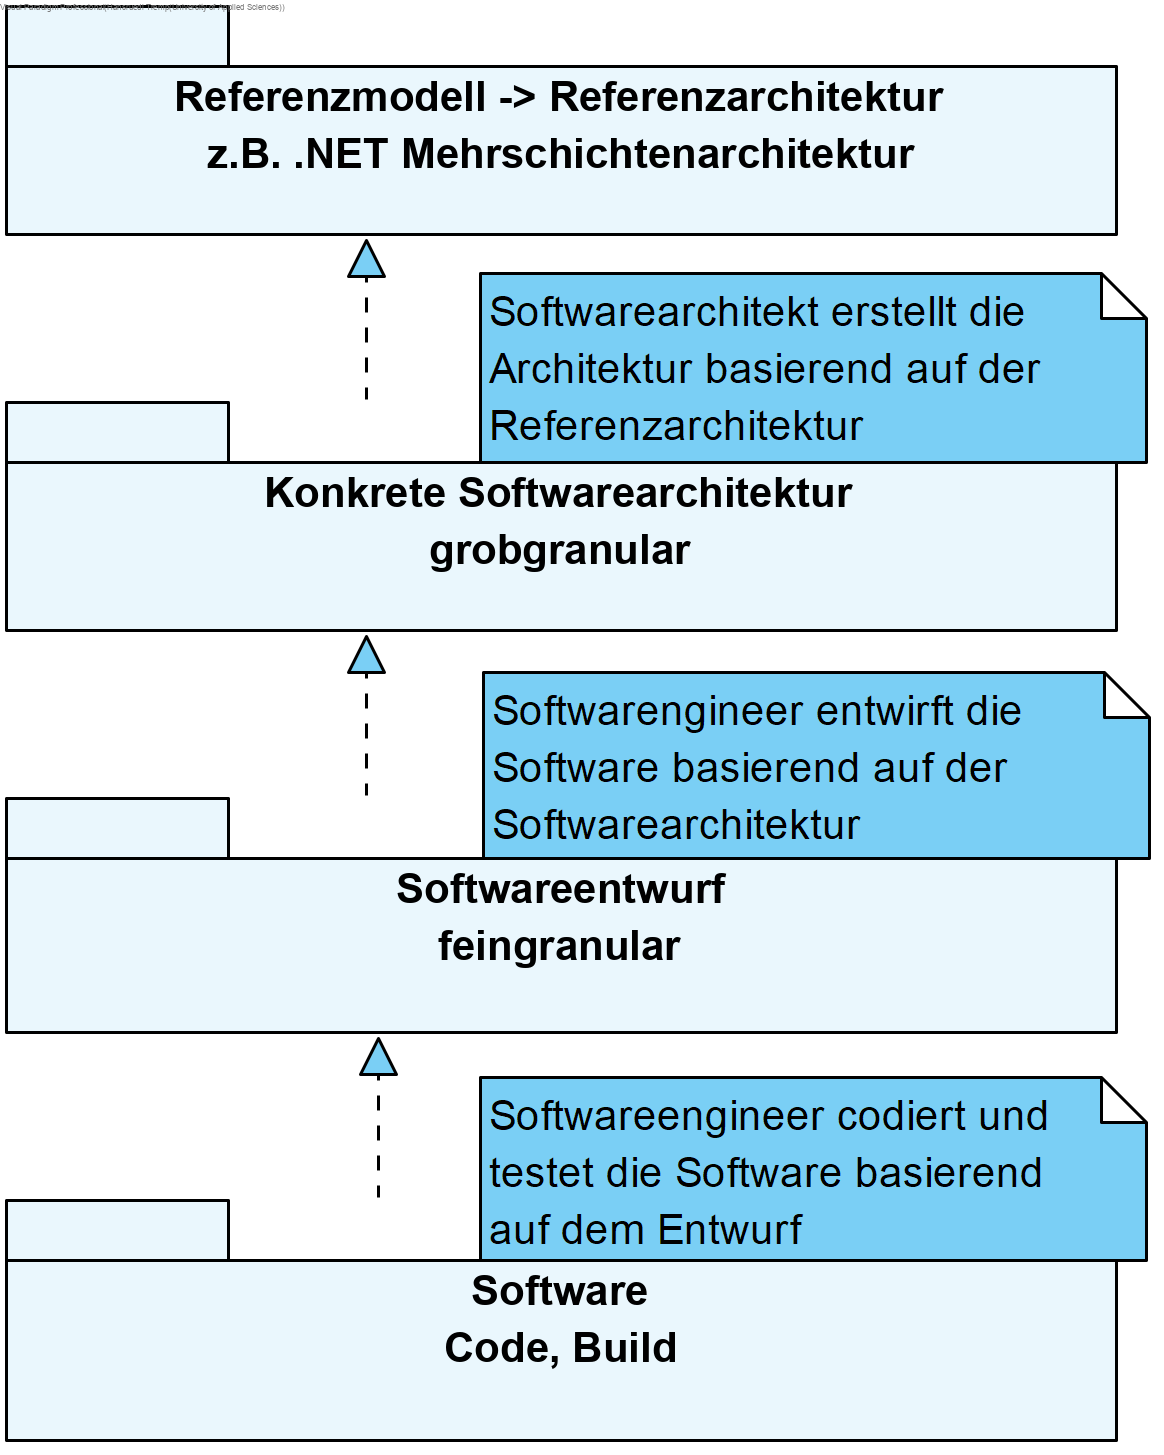
\includegraphics[width=0.7\linewidth]{introduction-arch-roles.png}

\subsubsection{Ebenen}

\textbf{Referenzmodell}

legt grundlegende Begriffe und Prinzipien fest (Bsp. .NET, Jakarta EE) \\

\textbf{Referenzarchitekturen}

Wenden \textcolor{blue}{Referenzmodelle} an und geben Musterarchitekturen vor (Bsp. Mehrschichtenarchitektur, IoT-Architektur) \\

\textbf{Softwarearchitektur} Wird basierend auf der
\textcolor{blue}{Referenzarchitektur} erstellt (Bsp. Mobile Native-App mit REST-Zugriff auf Web-Server), grobgranular, Darstellung oft mit \textcolor{blue}{UML-Klassendiagramm}

\textbf{Softwareentwurf}
Legt feingranulare Struktur fest (Bsp. Aufbau der Native-App: GUI - Funktionsebenen - Zugriff auf Server), feingranular, Darstellung oft mit \textcolor{blue}{UML-Klassendiagramm}

\subsubsection{Rollen}
\textbf{Enterprise/IT-Architekt}

Referenzmodell $\rightarrow$ Referenzarchitektur

\begin{itemize}
    \item Referenzmodell ist Leitfaden für Referenzarchitektur
    \item Baut Referenzarchitektur basierend auf dem Domänenverständnis des Referenzmodells
\end{itemize}
\vspace{10pt}
\textbf{Softwarearchitekt}

Referenzarchitektur $\rightarrow$ Konkrete Architekturen

\begin{itemize}
    \item Erstellt die Architektur basierend auf der Referenzarchitektur
    \item Legt grundlegende Strukturen fest
\end{itemize}
\vspace{10pt}
\textbf{Softwarengineer}

Konkrete Architekturen $\rightarrow$ Konkrete Systeme

\begin{itemize}
    \item Entwirft die Software basierend auf der Softwarearchitektur (grobgranular)
    \item Codiert und testet die Software basierend auf dem Entwurf (feingranular)

\end{itemize}

\subsubsection{Ziele}

\textbf{SMART}

\begin{itemize}
    \item \textcolor{blue}{Spezifisch}, konkret, fassbar
    \item \textcolor{blue}{Messbar}, testbar, später überprüfbar
    \item \textcolor{blue}{Akzeptiert} von (möglichst) allen Stakeholdern
    \item \textcolor{blue}{Realistisch}, aus aktueller Ressourcensicht machbar
    \item \textcolor{blue}{Terminiert} im Rahmen des Projektplanes
\end{itemize}
\vspace{10pt}
\textbf{Architekt (Person)}

Stabile \textcolor{blue}{Lösungskonzepte} für eine Reihe von technischen Aspekten liefern, damit Entwickler die Qualitätsziele erreichen. \\

\textbf{Architektur}

Ziel der Softwarearchitektur ist die Sicherstellung einer
adäquaten \textcolor{blue}{Softwareproduktequalität}.

\begin{itemize}
    \item \textcolor{blue}{Nützlichkeit} Applikation erfüllt ihre Funktionen
    \item \textcolor{blue}{Festigkeit} Software ist stabil und langlebig
    \item \textcolor{blue}{Ästhetik} User Experience ist ansprechend
\end{itemize}
\vspace{10pt}

\subsubsection{Anforderungen}
\textbf{Satzschablone}

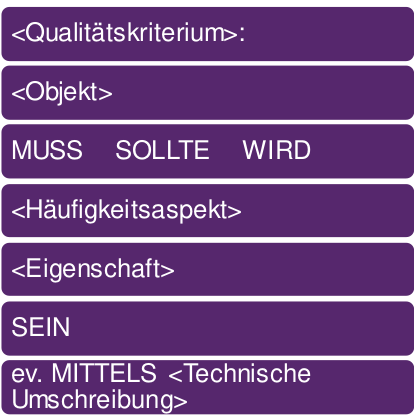
\includegraphics[width=0.6\linewidth]{introduction-satzschablone.png}

Beispiele
\begin{itemize}
    \item \textcolor{blue}{Verfügbarkeit} Das IT-System MUSS > 90 \% voll funktionstüchtig SEIN MITTELS passender Hardware und Netzwerkanbindung.
    \item \textcolor{blue}{Zeitverhalten} Die Antwort vom System MUSS in 80 \% der Fälle max. 2 Sec. SEIN
    \item \textcolor{blue}{Zeitverhalten} Die Antwort vom System SOLLTE in 90 \% der Fälle max. 1 Sec SEIN
    \item \textcolor{blue}{Interoperabilität} Das Austauschformat zwischen den Microservices WIRD immer JSON SEIN.
\end{itemize}
\vspace{10pt}
\textbf{ISO 25010 Softwarequalitätsmodell}

Benutzer

\begin{itemize}
    \item Funktionalität
    \item Performance und Effizienz
    \item Kompatibilität und Interoperabilität
    \item Benutzbarkeit
    \item Verfügbarkeit
\end{itemize}

Betreiber/Entwickler

\begin{itemize}
    \item IT-Sicherheit
    \item Warbarkeit
    \item Portierbarkeit
\end{itemize}


\subsubsection{Struktur (Modellierung)}

Hilft für

\begin{itemize}
    \item Beherrschung der Komplexität
    \item Architektur gestalten und kommunizieren
    \item Verständigung mit Stakeholdern
    \item Dokumentation und Nachvollziehbarkeit gewährleisten
\end{itemize}
\vspace{10pt}
\textbf{Bausteine}

\begin{itemize}
    \item \textcolor{blue}{Pakete} Fassen untergeordnete Pakete bzw. Komponenten zu einer Einheit zusammen (Bsp. in Schichten).
    \item \textcolor{blue}{Komponenten} Klar definiertes Verhalten und bieten Schnittstellen an oder Konsumieren diese über Beziehungen
\end{itemize}
\vspace{10pt}
\textbf{Diagramme}

\textcolor{blue}{Kontextsicht} zeigt den Scope des Systems mit den Schnittstellen

\begin{itemize}
    \item Kontextdiagramm \\
    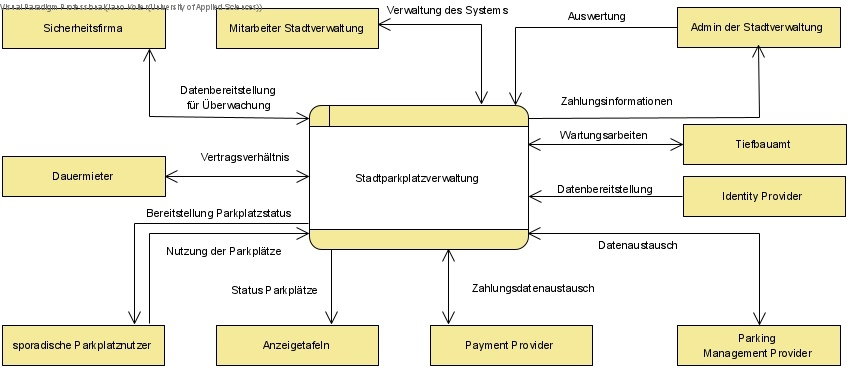
\includegraphics[width=\linewidth]{introduction-context-diagram.png}
    \item Use Case Diagramm
\end{itemize}

\textcolor{blue}{Bausteinsicht} zeigt strukturellen Aufbau des Systems

\textcolor{blue}{Laufzeitsicht} zeigt dynamische Aspekte, wie Interkation, Prozessablauf und Verhalten

\begin{itemize}
    \item Sequenzdiagramm
    \item Aktivitätsdiagramm
    \item Zustandsdiagramm
\end{itemize}

\textcolor{blue}{Verteilungssicht} zeigt die Verteilung der Softwareartefakte in der IT-Infrastruktur

\begin{itemize}
    \item Deployment Diagram
\end{itemize}

\subsubsection{Prüfungsfragen}

\begin{itemize}
    \item Erläutern Sie die Aufgabe der Softwarearchitektur im Rahmen eines Softwareentwicklungsprojektes! \\
    \textcolor{blue}{Der Softwarearchitekt gibt anhand
    einer Referenzarchitektur die Architekturvorgaben. Er hilft unteranderem mit, die Architekturrichtlinien und -standards in der IT-Strategy zu entwickeln. Zusätzlich ist der für die Kommunikation mit den Stakeholdern zuständig.}
    \item Welche Beziehung hat die Softwarearchitektur zur Referenzarchitektur einerseits und dem Softwarentwurf andererseits? \\
    \textcolor{blue}{Die Softwarearchitektur ist eine konkrete Anwendung einer Referenzarchitektur und bildet die Vorlage für den feingranularen Softwareentwurf.}
    \item Welche konkreten Artefakte erstellt der Softwa-
    rearchitekt? \\
    \textcolor{red}{Antwort}
    \item Welches sind die drei Hauptziele in der Analogie mit der klassischen Bauarchitektur? \\
    \textcolor{blue}{Nützlichkeit, Festigkeit, Ästhetik}
    \item Wozu dient arc42? \\
    \textcolor{blue}{Vorlage für die Dokumentation}
    \item Mit welchem Diagrammtyp von UML können sie die Struktur eines Softwaresystems beschreiben? \\
    \textcolor{blue}{Komponentendiagramm}
    \item Wozu dient ein UML Komponentendiagramm? \\
    \textcolor{blue}{Darstellung des strukturellen Aufbaus, sowie die Beziehungen der Komponenten}
    \item Nennen Sie drei der wichtigsten Werkzeuge eines Softwarearchitekten! \\
    \textcolor{blue}{Wiki, Modellierungstools, Analysetools und Testtools}
\end{itemize}

        \vfill\null
        \columnbreak
        \subsection{Serviceorientierte Architektur (SOA)}

\textbf{Service (Dienst)}

Angebot einer Geschäftsprozess oder IT-Dienstleistung, Zugriff über eine klar geregelte Schnittstelle (Interface)

\subsubsection{Grundprinzipien}

\begin{itemize}
    \item \textcolor{blue}{Geschäftsrelevante Services} bildet meist eine Teilfunktion eines Geschäftsprozesses
    \item \textcolor{blue}{Service Kontrakt: Service Level Agreement (SLA)} Inhalt/Zweck der Leistungserbringung, QoS (Quality of Service wie z.B. Verfügbarkeit, Performanz usw.), Zugriff (Authentisierung, Autorisierung), Support, Kosten, Sanktionen
    \item \textcolor{blue}{Service Auffindbarkeit} Service ist in einem Verzeichnis registriert
    \item \textcolor{blue}{Servicekomposition} Mehrere Services können z.B. im Rahmen eines Geschäftsprozesses im Workflow komponiert werden
\end{itemize}

\subsubsection{Service Lifecycle}

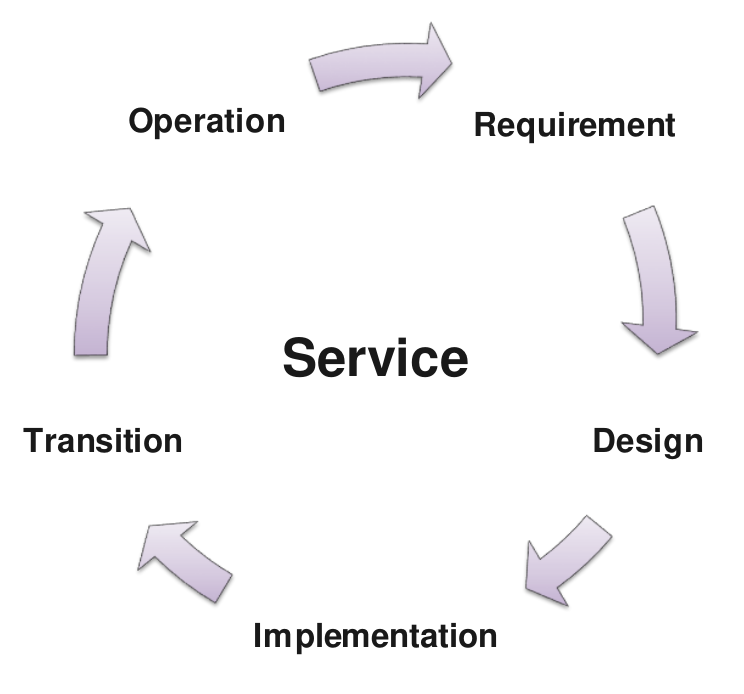
\includegraphics[width=0.6\linewidth]{soa-service-lifecycle.png}

\begin{enumerate}
    \item \textcolor{blue}{Requirements} Aufnahme der Anforderungen
    und Abstimmung mit den Stakeholdern
    \item \textcolor{blue}{Design} Serviceengineer beschreibt API, Funktionalität, Konfigurierbarkeit usw. und legt das SLA mit den Konsumenten fest.
    \item \textcolor{blue}{Implementation} Softwareentwickler implementiert den Service
    \item \textcolor{blue}{Transition} (Einführung) Installation, Publikation im Dienstverzeichnis, sowie Information bzw. Instruktion für betreffende Stakeholder
    \item \textcolor{blue}{Operation} Nutzung mit fortlaufendem Monitoring $\rightarrow$ neue Anforderungen zur Optimierung oder Erweiterung
\end{enumerate}

\subsubsection{Fundamentales SOA-Dreieck}

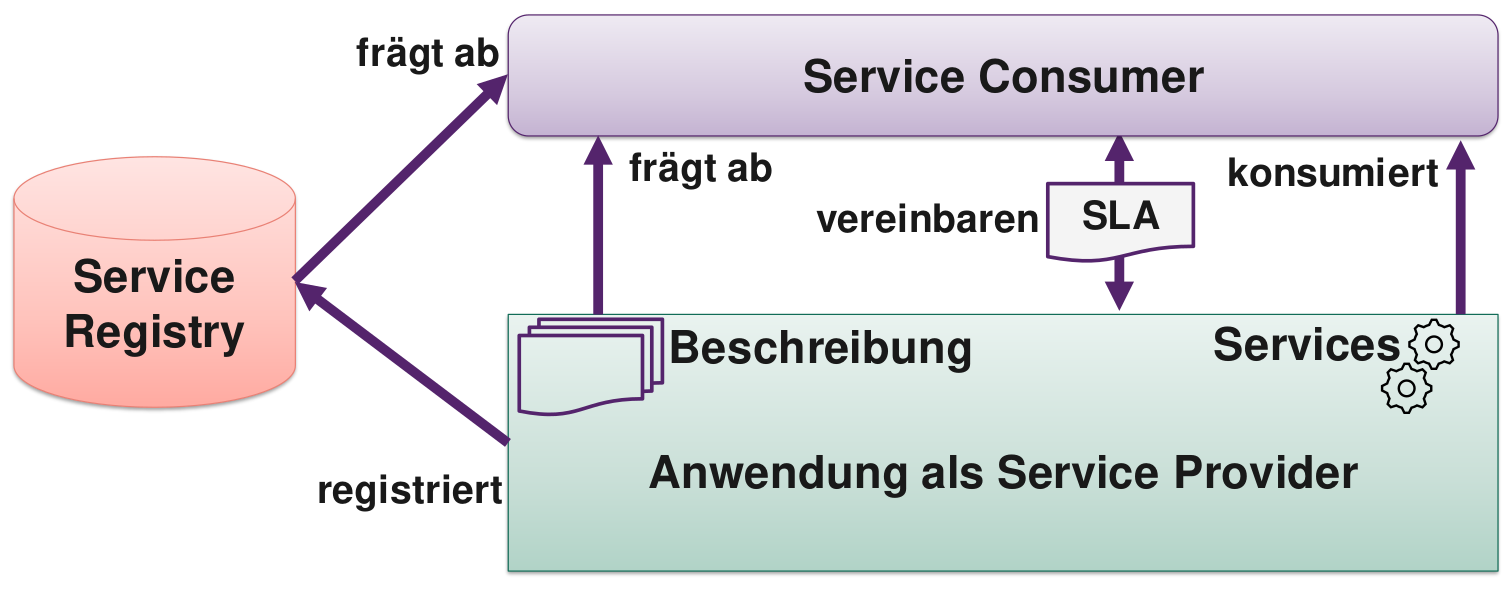
\includegraphics[width=\linewidth]{soa-soa-dreieck.png}

\columnbreak
\subsubsection{Service Modellierung (SoaML)}

\textbf{Service-oriented architecture Modeling Language (SoaML)}

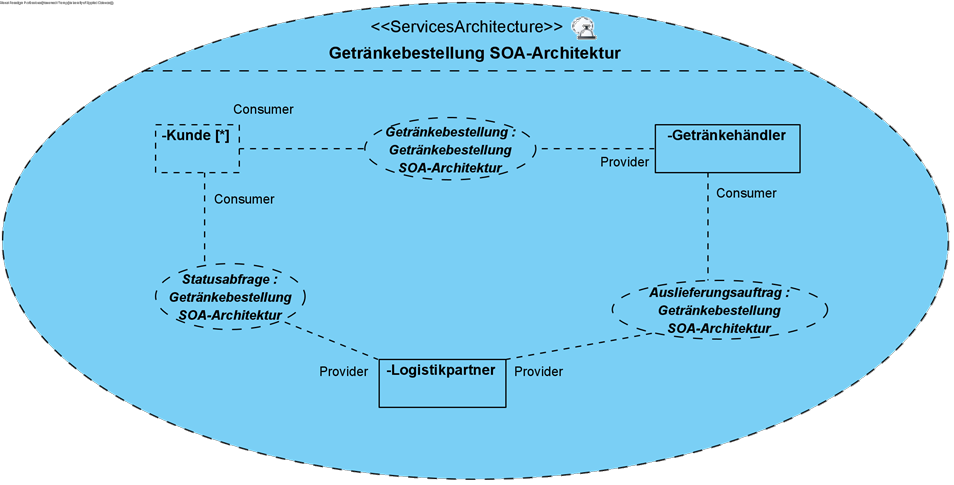
\includegraphics[width=\linewidth]{soa-modeling.png} \\

Beispiel

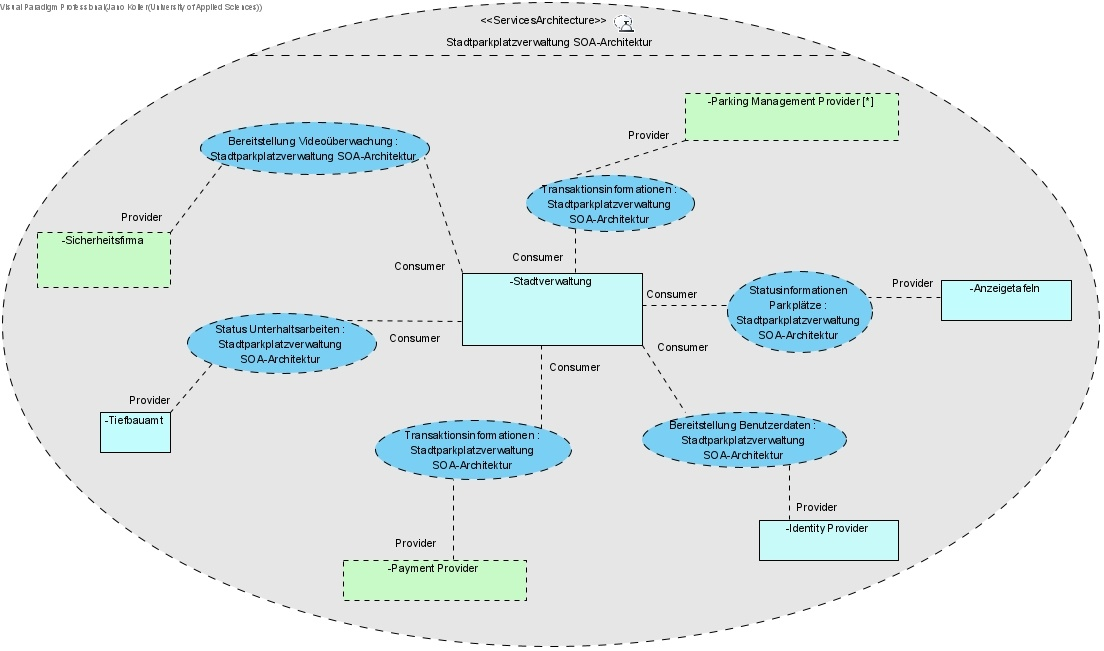
\includegraphics[width=\linewidth]{soa-example.png} \\

\textbf{Sequenzdiagramm}

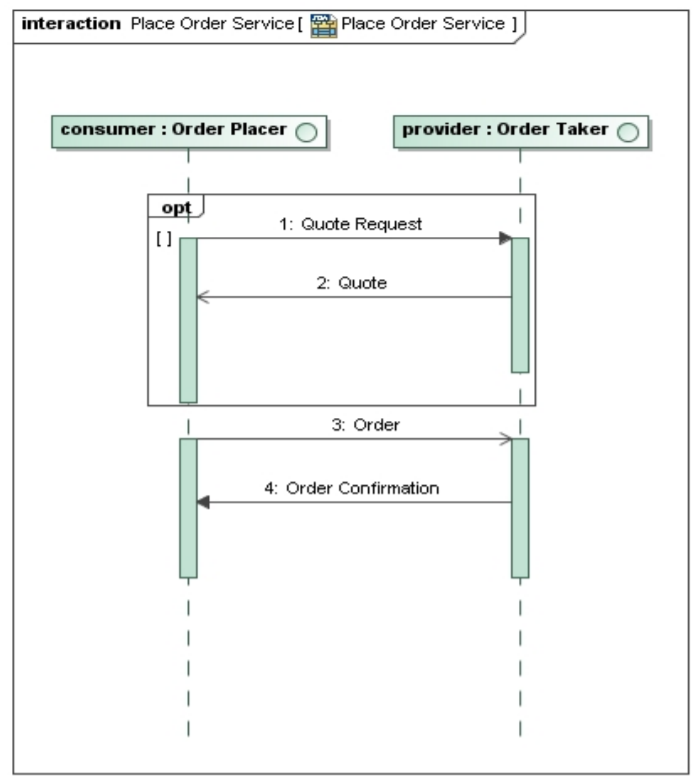
\includegraphics[width=0.7\linewidth]{soa-sequence-diagram.png}

\columnbreak
\subsubsection{Synchrone Web Services}

\textbf{SOAP}

Simple Object Access Protocol, zustandsbehaftet, ruft Funktionen bzw. Methoden auf, mit der WSDL (Web Service Description Language) werden Schnittstellen beschrieben, funktioniert auf Anwendungsebene folgendermassen

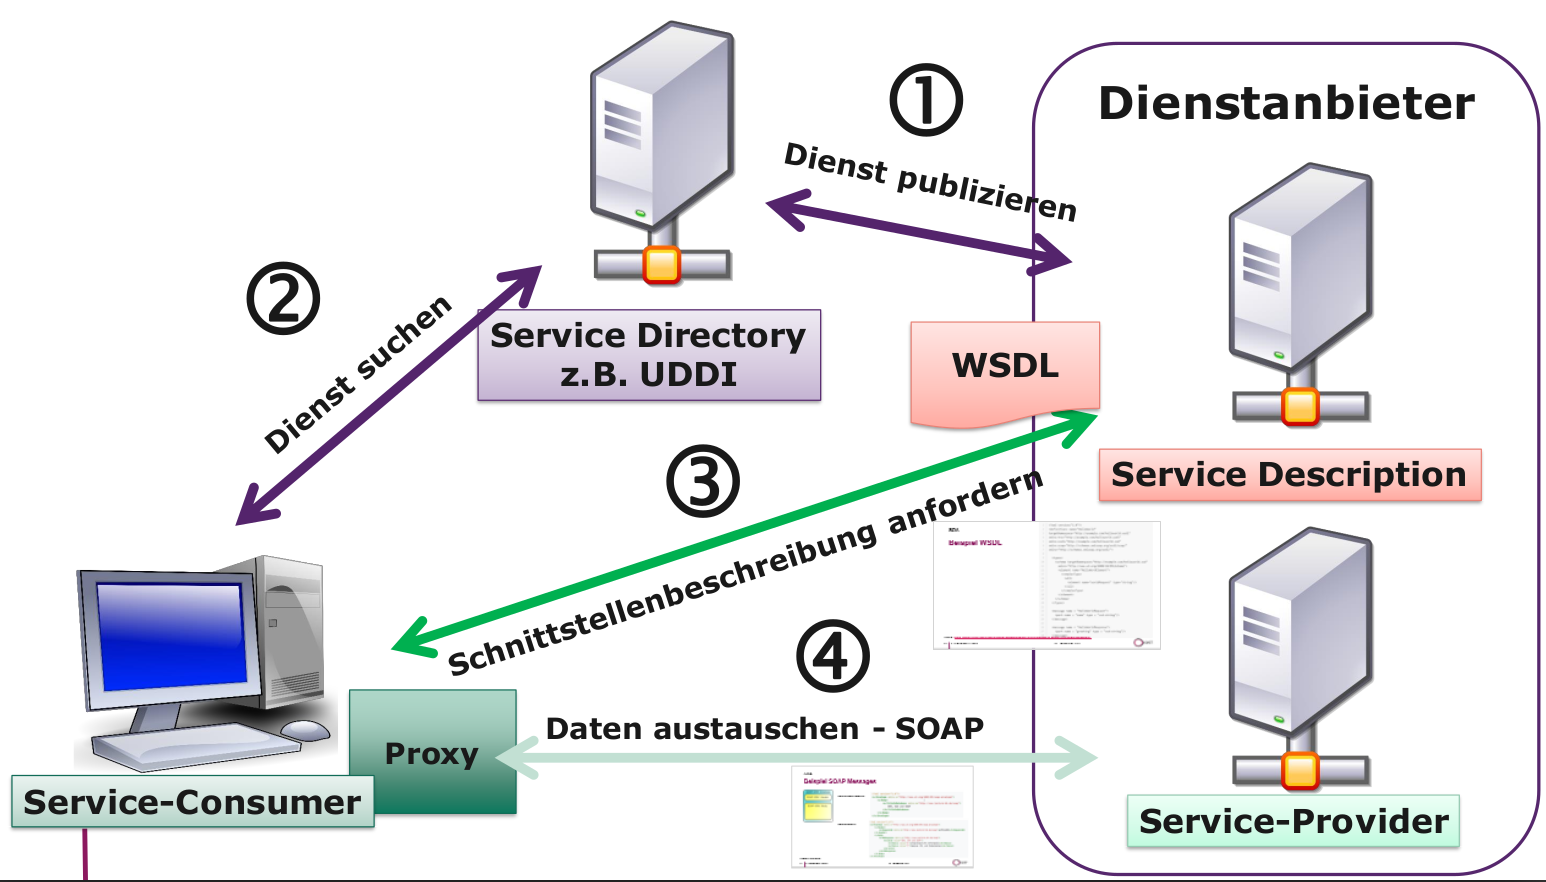
\includegraphics[width=\linewidth]{soa-soap.png}

\begin{enumerate}
    \item Service-Provider publiziert SOAP-Dienst beim Service Directory, basiert bspw. auf UDDI (universal Description, Discovery and Integration)
    \item Service-Consumer sucht in Service Directory nach dem Service und erhält URI für Schnittstellenbeschreibung
    \item Mit der aufgerufenen WSDL-Beschreibung kann Consumer-Runtime den Proxy automatisch erstellen
    \item Proxy fungiert als Adapter, um die Methoden des SOAP-Services ansprechen zu können
\end{enumerate}
\vspace{10pt}
\textbf{REST}

Representational State Transfer, ressourcenorientiert, zustandslos, verwendet HTTP-Befehle, Payload ist meist JSON, kann aber auch XML oder anders Format sein, hat keine standardisierte Schnittstellenbeschreibung


\begin{itemize}
    \item \textcolor{blue}{GET} Ressource(n) [z.B. Kunde(n)] anfordern
    \item \textcolor{blue}{POST} einfügen einer Ressource (z.B. Kunde), senden einer Message
    \item \textcolor{blue}{PUT} ändern einer Ressource
    \item \textcolor{blue}{MERGE} Teil einer Ressource ändern
    \item \textcolor{blue}{DELETE} löschen einer Ressource
\end{itemize}
\vspace{10pt}
\textbf{OData}

REST-basierter flexibler Datendienst, basiert auf Metadaten, Bietet Datenressourcen und Funktionen an, Payload ist JSON oder AtomPub (XML) \\

\textbf{GraphQL}

Query-Sprache, erlaubt gezielte Bearbeitung von Daten, Schema Definition Language, kann Daten aus mehreren Ressourcen zusammennehmen, Arbeitet mit HTTP - POST

\columnbreak
\subsubsection{Asynchrone Kommunikation}

Kommunikation mittels Nachrichten (Messages), Sender und Empfänger sind zeitlich entkoppelt, ermöglicht hohe Parallelität mit geringen Ressourcenverbrauch, \textcolor{blue}{Kommunikation mittels Message Oriented Middleware (MOM)} \\

Vorteile

\begin{itemize}
    \item lose Kopplung zwischen Applikationen
    \item hohe Fehlertoleranz
    \item geringer Ressourcenverbrauch
    \item schnelle parallele Verarbeitung
    \item dynamische Skalierung
    \item hohe Flexibilität bei Änderungen
\end{itemize}

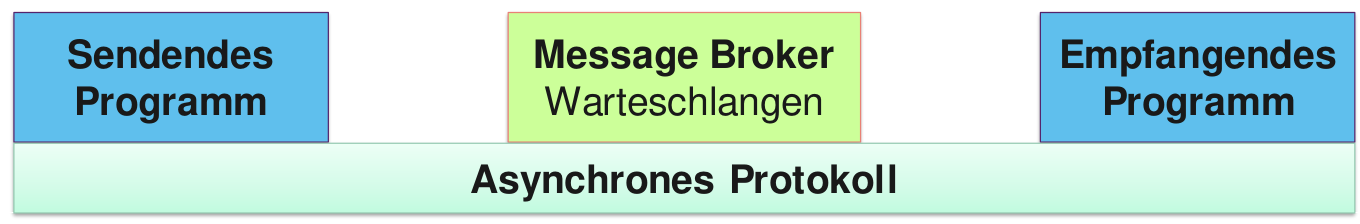
\includegraphics[width=\linewidth]{soa-mom.png}

\textbf{Protokolle}

\textcolor{blue}{AMQP} Advanced Message Queuing Protocol ist ein standardisiertes asynchrones Message-Protokoll zur Kommunikation zwischen Client und Message Broker sowie zwischen unterschiedlichen Message Brokern.

\textcolor{blue}{MQTT} für IoT \\

\textbf{Message Broker}

verwaltet diverse Queues. Er vermittelt und speichert die erhaltenen Nachrichten un untersützt unterschiedliche Kommunikationsmuster.

\textcolor{blue}{RabbitMQ} Open Source, Message Store, Message Passing (One-Way) oder Request-Reply

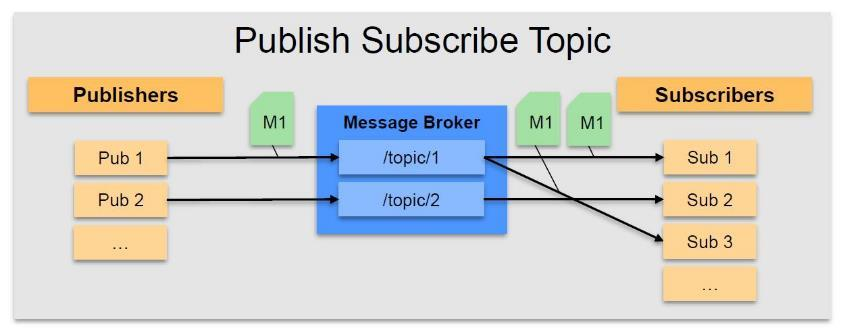
\includegraphics[width=0.8\linewidth]{soa-rabbitmq-1.png}

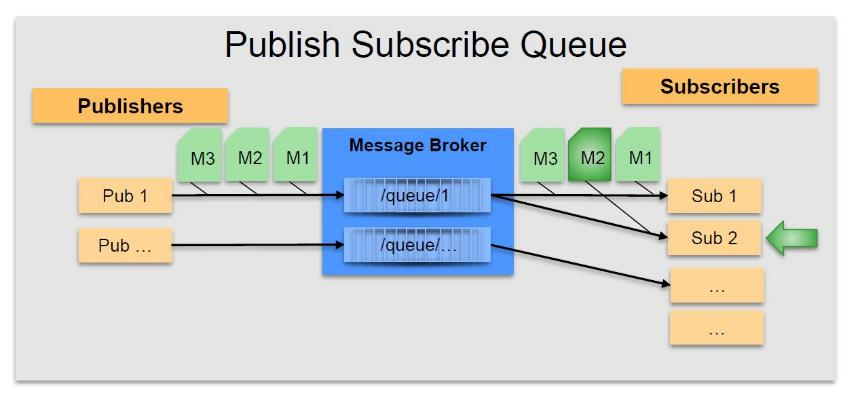
\includegraphics[width=0.8\linewidth]{soa-rabbitmq-2.png} \\

Publish
\begin{lstlisting}
asyncapi: 2.2.0
info:
  title: Hello world application
  version: '0.1.0'
channels:
  hello:
    publish:
      message:
        payload:
          type: string
          pattern: '^hello .+$'
\end{lstlisting}
\vspace{10pt}
\columnbreak
Subscribe
\begin{lstlisting}
asyncapi: 2.2.0
info:
  title: Example
  version: 0.1.0
channels:
  user/signedup:
    subscribe:
      message:
        description: An event describing
        payload:
          type: object
          additionalProperties: false
          properties:
            fullName:
              type: string
            email:
              type: string
              format: email
            age:
              type: integer
              minimum: 18
\end{lstlisting}

\subsubsection{Elektronische Nachricht}

\textbf{1. Ebene: Semantik}

Inhaltliche Bedeutung (im Anwendungskontext)

\begin{itemize}
    \item \textcolor{blue}{Nachrichtentyp} Bsp. Offer, Order, Invoice
    \item \textcolor{blue}{Basisstruktur} Bedeutung einzelner Felder, Datentyp, Codetabellen, gültige Werte
\end{itemize}

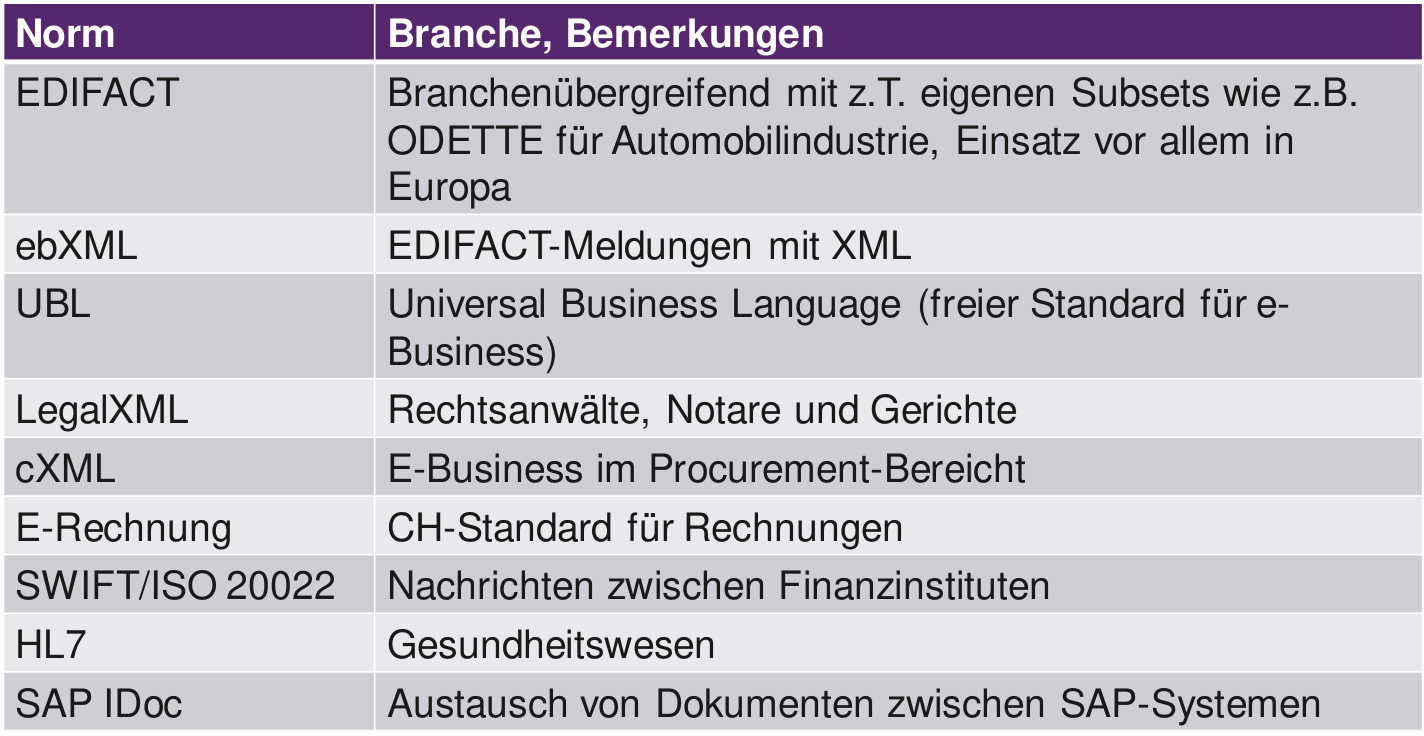
\includegraphics[width=\linewidth]{soa-semantic.png} \\


\textbf{2. Ebene: Format}

Technischer Aufbau/Struktur einer Nachricht

\begin{itemize}
    \item \textcolor{blue}{CSV} Comma Separated Values, kompakt, plattformspezifisch
    \item \textcolor{blue}{EDI} Electronic Data Interchange, klassische» EDIFACT-Meldungen, E-Business, branchenübergreifend
    \item \textcolor{blue}{XML} Extended Markup Language, gibt bis zu 50 \% Overhead, plattformunabhängig, HTML für E-Mail
    \item \textcolor{blue}{JSON} JavaScript Object Notation, kompakter als XML, bei RESTful-Services beliebt
\end{itemize}
\vspace{10pt}
\textbf{3. Ebene: Codierung}

Definiert die verwendete Codetabelle für die Bitfolgen je Zeichen, Bitfolge für die Festlegung der Zeichen

\begin{itemize}
    \item \textcolor{blue}{ASCII} ANSI-Standard
    \item \textcolor{blue}{EBCDIC} IBM-Standard
    \item \textcolor{blue}{Unicode} internationaler Standard, jedes Zeichen in der Welt hat eine fixe Bitkombination: 8 / 16 oder 32 bit, UTF-8
\end{itemize}

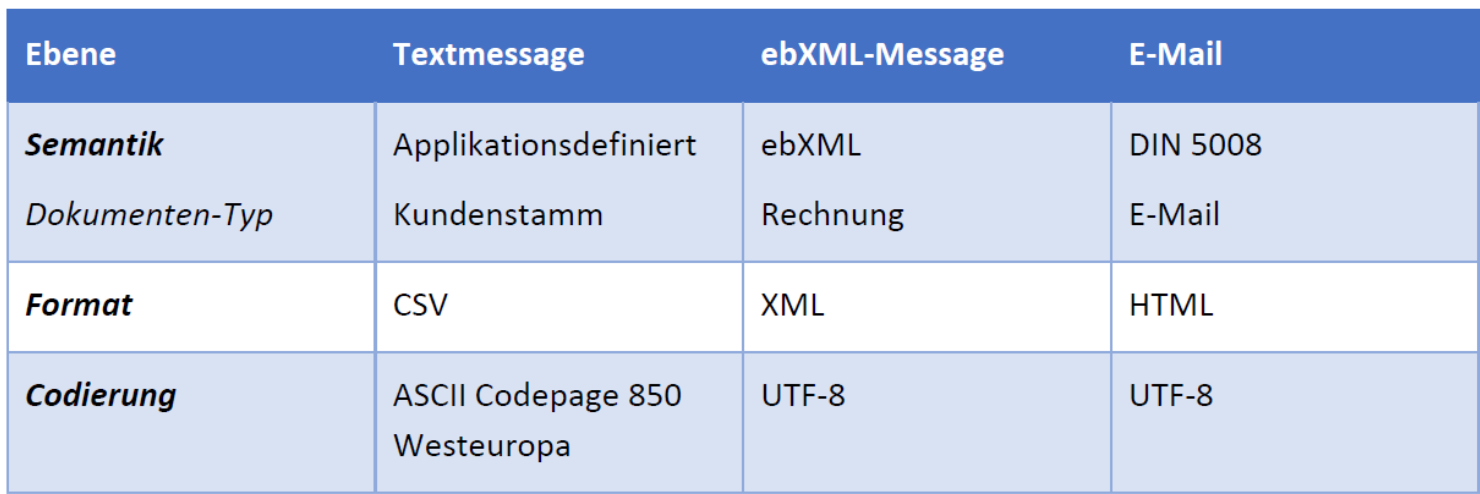
\includegraphics[width=\linewidth]{soa-message-example.png}

\subsubsection{IT-Sicherheit}

\textbf{Schutzziele}

\begin{itemize}
    \item \textcolor{blue}{Vertraulichkeit} Unbefugter Informationsgewinn
    \item \textcolor{blue}{Integrität} Unbefugte Modifikation (Änderung) von Daten bzw. Funktionen
    \item \textcolor{blue}{Verfügbarkeit} Unbefugte Beeinträchtigung der Funktionalität bzw. Verfügbarkeit
    \item \textcolor{blue}{Nachweisbarkeit} Nachvollziehbarkeit bzw. Nichtabstreitbarkeit einer Handlung
\end{itemize}
\vspace{10pt}
\textbf{Zugriffssicherheit}

Schutz vor unerlaubter Nutzung

SSO (Single Sign On) Lösungen
\begin{itemize}
    \item \textcolor{blue}{SAML} Security Assertion Markup Language
    \item \textcolor{blue}{OAuth 2.0} für Webservices, Token orientiert
\end{itemize}
\vspace{10pt}
\textbf{Messagesicherheit}

End-zu-End Verschlüsselung

\begin{itemize}
    \item \textcolor{blue}{XML-Message Security} XML Encryption (Verschlüsselung der XML-Nachricht), XML Signature (Digitales signieren einer XML-Nachricht)
    \item \textcolor{blue}{E-Mail Security} S-/MIME, PGP
\end{itemize}


\subsubsection{API Entwicklung}

\begin{enumerate}
    \item \textcolor{blue}{Service Requirements} Anforderungen an den Service im Detail festlegen
    \item \textcolor{blue}{Design} Entwickler entwirft einzusetzende Technologien, Funktionsumfang, Inhalte und Integration der API
    \item \textcolor{blue}{Mocking (Prototype)} Entwickler erstellt mit dem Spezifikationen einen Prototypen
    \item \textcolor{blue}{Validate} Mit dem Mockup-Service validiert Entwickler die Schnittstelle mit den Stakeholdern
    \item \textcolor{blue}{Build} Entwicklung der API und Integration mit dem Backend
    \item \textcolor{blue}{Document} Dokumentation der Verwendung der API
    \item \textcolor{blue}{Test} Nachweis für die korrekte Funktionalität und QoS
    \item \textcolor{blue}{Deploy and Publish} Verteilung der API auf Zielplattform und Publikation im Service Directory
    \item \textcolor{blue}{Monitor} Überwachung der Nutzung der API
\end{enumerate}

\subsubsection{API Management}

\textbf{Funktionen}

\begin{itemize}
    \item \textcolor{blue}{API Lifecycle Management} Sicherstellung der Konsistenz zwischen verschiedenen Versionen
    \item \textcolor{blue}{API-Governance (Einhalten von Policies [Richtlinien])}
    \item \textcolor{blue}{API-Sicherheit} SSL Offloading, Authentisierung zum Schutz der API vor Missbrauch
    \item \textcolor{blue}{Automatisiertes API-Deployment und Publishing} anhand Policies
    \item \textcolor{blue}{API-Gateway mit Load-Balancing und Fault-Tolerance} Sicherstellung einer optimalen Performance durch Caching, Skalierung, Load-Balancing und Fehlertoleranz
    \item \textcolor{blue}{API-Monitoring und Analytics} Monitoring und automatisches Logging für die Überwachung
\end{itemize}

\columnbreak
\subsubsection{Prüfungsfragen}

\begin{itemize}
    \item Was ist das Hauptmerkmal von SOA? \\
    \textcolor{blue}{Bereitstellung von unterschiedlichen
    Services}
    \item Welches sind die drei Schnittstellen eines Service? Erläutern Sie stichwortartig deren Funktion \\
    \textcolor{blue}{Control API, API, und Point of Observation}
    \item Welches sind die fünf Prozessschritte des Service-Lifecycle? \\
    \textcolor{blue}{Requirement, Design, Implementation, Transition, Operation}
    \item Zeichnen Sie das fundamentale SOA-Dreieck mit dessen Komponenten und Interaktionen auf \\
    \textcolor{blue}{Siehe 2.2 SOA-Dreieck}
    \item Welcher Diagrammtyp von SoaML eignet sich für die Kommunikation der Serviceübersicht? \\
    \textcolor{blue}{Service Architecture Diagram}
    \item Zeichnen Sie den Protokollstack einer SOAP-Kommunikation auf \\
    \textcolor{blue}{Envelope (defines message structure), set of encoding rules,     convention for RPC and responses}
    \item Was ist der Vorteil von GraphQL gegenüber REST? \\
    \textcolor{blue}{GraphQL fragt, im Gegensatz zu REST, dynamisch nur die benötigten Objekte und Attribute ab. Serverseitige Applikation wird wie eine Datenbank behandelt.}
    \item Welche Kommunikationsmuster unterstützt ein Message Broker? \\
    \textcolor{blue}{Message Passing, Request-Reply, Publish-Subscribe Topic, Publish-Subscribe FI-FO}
    \item Welche Themen definiert UBL? \\
    \textcolor{red}{Antwort}
    \item Welches Autorisierungsprotokoll würden Sie für einen RESTful-Service einsetzen? \\
    \textcolor{blue}{OAuth 2.0}
    \item Wozu dient XML Signature? \\
    \textcolor{blue}{Damit man sicher sein kann, von wem die Nachricht stammt}
\end{itemize}


        \newpage
        \section{Mehrschichten-Softwarearchitektur}
        \begin{itemize}
    \item \textcolor{blue}{Provider} Server, welche Services anbieten
    \item \textcolor{blue}{Consumer} sind Clients oder Server, die Services beziehen/benötigen
\end{itemize}

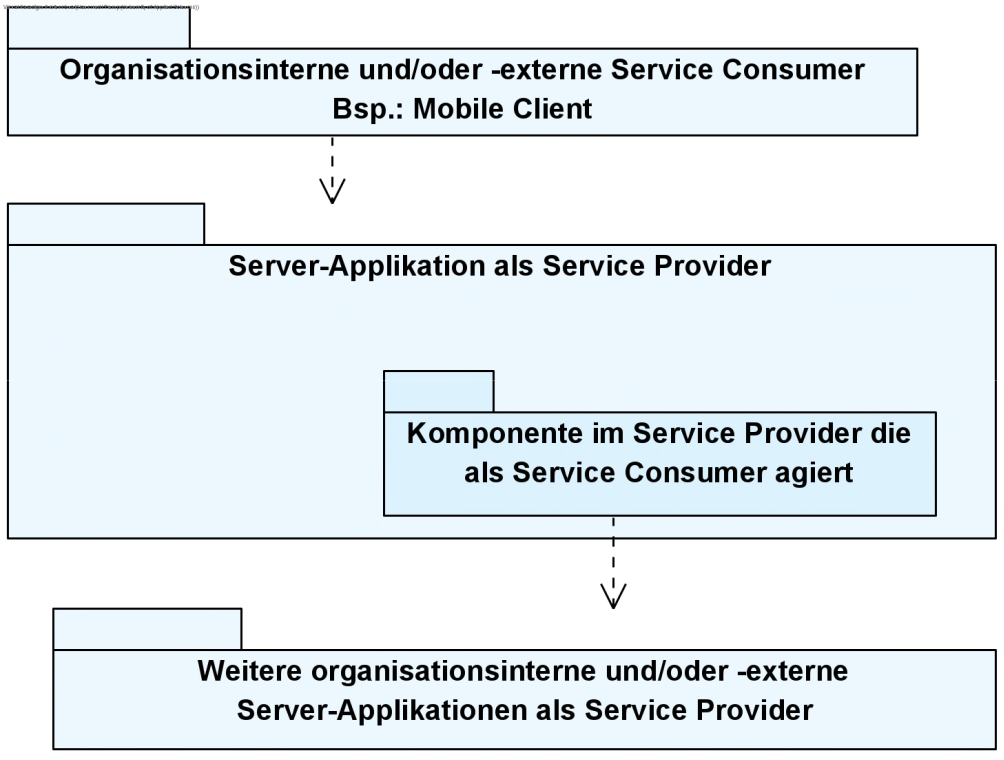
\includegraphics[width=\linewidth]{introduction2-client-server-model.png}


\subsection{SOA-enabled Mehrschichtenarchitektur (N-Tier-Architecture)}

\subsubsection{Client-/Front-End-Tier (Layer)}

Ermöglicht dem Anwender die Interaktion mit dem IT-System über eine Benutzerschnittstelle

\begin{itemize}
    \item Container: Web Browser for Web Apps
\end{itemize}

\subsubsection{Server Tiers (Layers)}

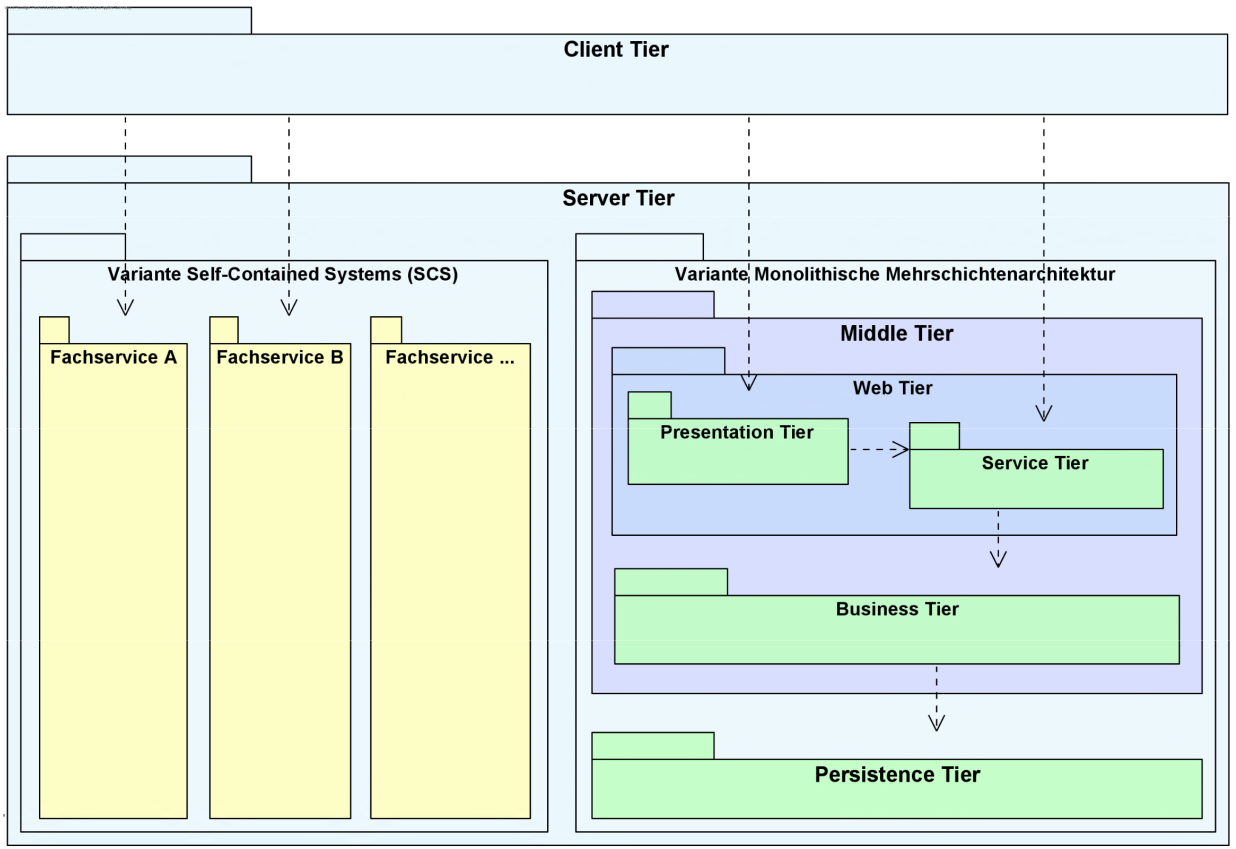
\includegraphics[width=\linewidth]{introduction2-client-server-tiers.png}

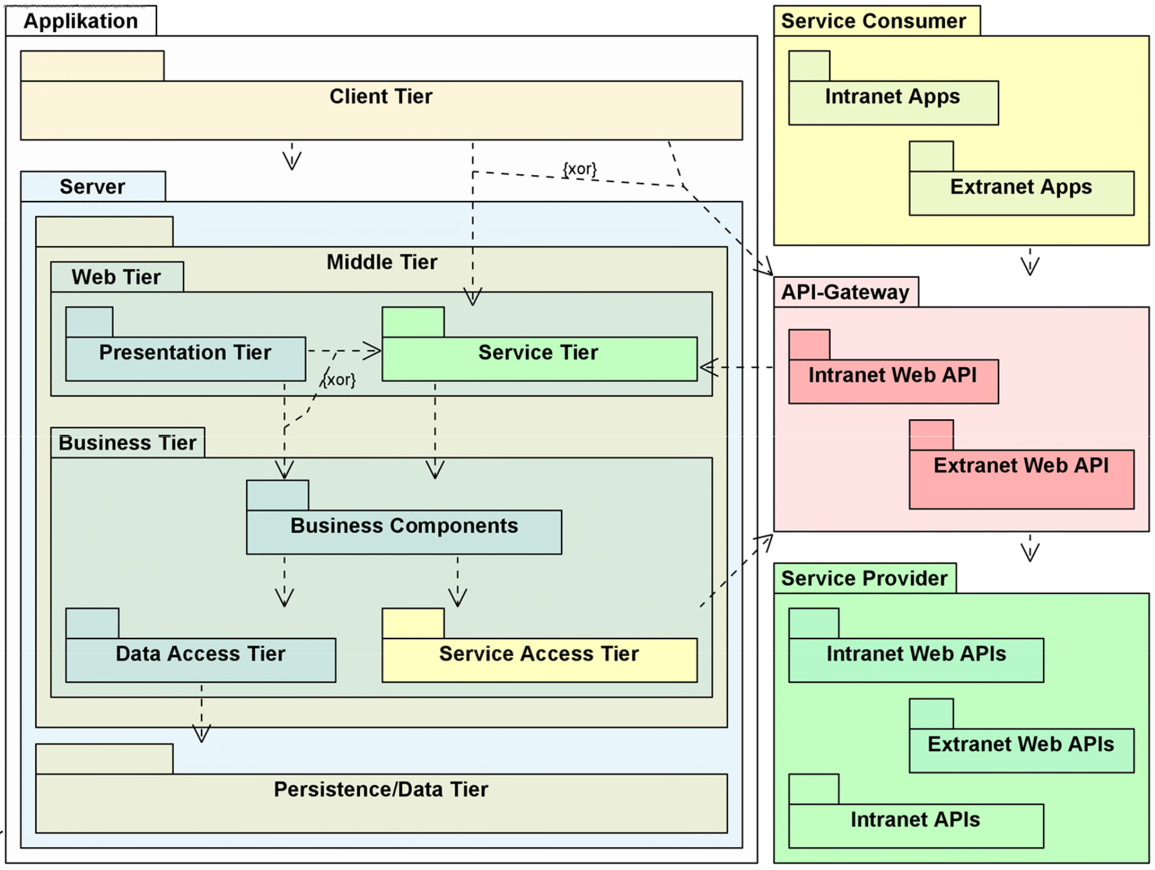
\includegraphics[width=\linewidth]{introduction2-n-tier-architecture.png} \\

\textbf{Middle-/Business-Tier (Layer)}

\begin{itemize}
    \item \textcolor{blue}{Web Tier} Präsentation, Services, bietet die Schnittstelle zum Server an
        \begin{itemize}
            \item \textcolor{blue}{Presentation Tier} Für Web Apps, welche die  View-Aufbereitung auf dem Server vornehmen. Interagiert mit dem Webbrowser.
            \item \textcolor{blue}{Service Tier} Zugriff über Web API für Service Consumer geben, meist REST oder neuerdings GraphQL, vorgelagertes API-Gateway, bildet die Service-Zugriffsebene von ausserhalb der Applikation. Damit lassen sich anderen gezielt Daten oder Funktionalität zur Verfügung stellen.
        \end{itemize}
    \item \textcolor{blue}{Business Tier} Facade für kontrollierten Zugriff, Herzstück: Business Components / Businesslogik, enthält die Geschäftslogik
        \begin{itemize}
            \item \textcolor{blue}{Data Access Tier} Access Facade, trennt sauber die in der betreffenden Fachapplikation gehaltene Persistenz, Entkoppelung der Business Komponente von DBMS-spezifischem Code (Bsp. .NEt Entity Framework)
            \item \textcolor{blue}{Service Access Tier} entkoppelt externe Service-Schnittstellen von den Business-Komponenten. Kann direkt oder über API-Gateway auf Service Provider zugreifen. Hier ist je aufgerufene externe Schnittstelle eine Proxy-Komponente zu entwickeln.
        \end{itemize}
\end{itemize}
\vspace{10pt}
\textbf{Data-/Persistence-Tier (Layer)}

speichert die Datenobjekte, hält Datenobjekte persistent, Datenbank Management(system)

\begin{itemize}
    \item \textcolor{blue}{CRUD Model} Create-Read-Update-Delete \\
    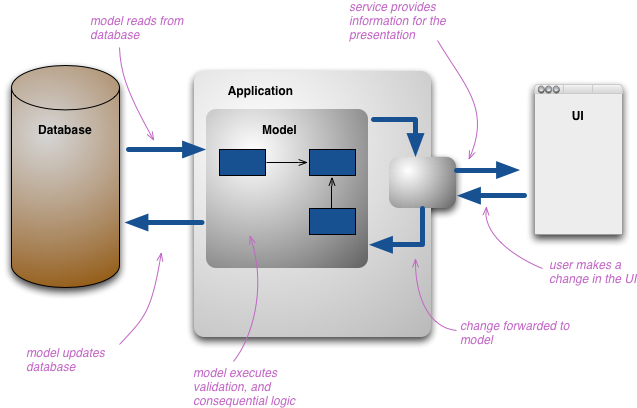
\includegraphics[width=\linewidth]{introduction2-crud}
    \item \textcolor{blue}{CQRS} Command Query Separation \\
    Das System trennt abfragenden von verändernden DB-Befehlen. Read-Befehle werden in einem Query Handler verarbeitet und in einer replizierten DB-Instanz ausgeführt, CUD-Befehle werden vom Command Handler verarbeitet und im Primary DBMS (exklusiv für verändernde Befehle) ausgeführt. \\
    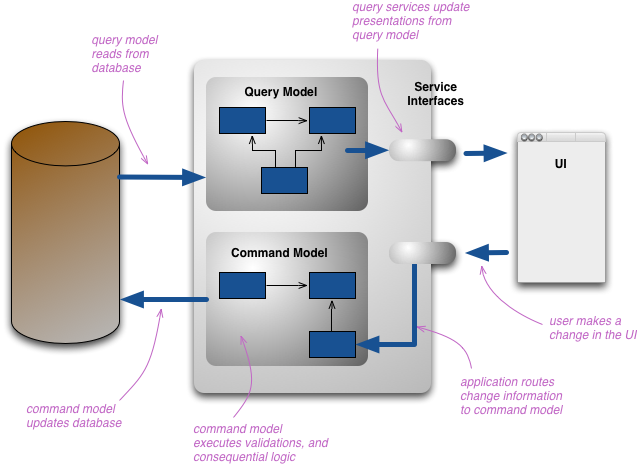
\includegraphics[width=\linewidth]{introduction2-cqrs.png}
\end{itemize}
\vspace{10pt}
\textbf{Event Sourcing (ES)}

ein Verfahren, bei dem alle Veränderungen des Zustands einer Softwareanwendung als Sequenz von Events abgebildet und aufgezeichnet werden. Er holt sich das nächste verfügbare DB-
Ereignis, um die entsprechenden DB-Befehle in der Primary DBMS ausführen zu lassen. Sobald der SQL-Befehl erfolgreich verarbeitet wurde, holt er den nächsten Befehl usw.

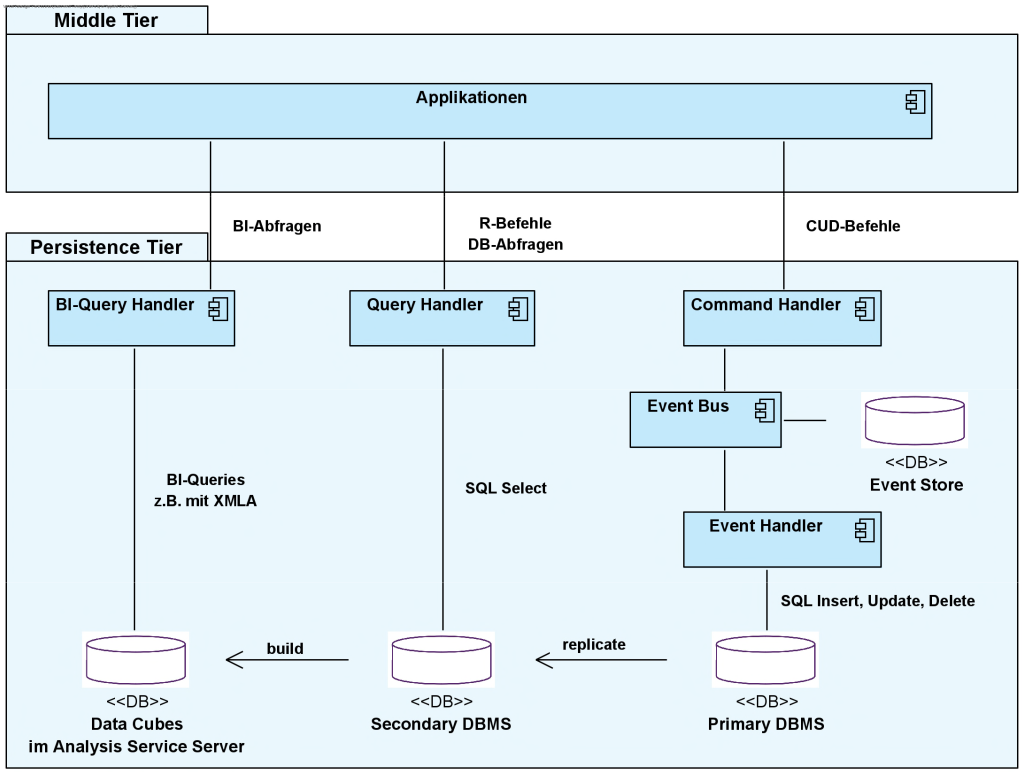
\includegraphics[width=\linewidth]{introduction2-es.png}

\subsection{Cloud}

\begin{itemize}
    \item Kosten fallen gemäss den reservierten oder effektiv genutzten Ressourcen an
    \item IT wächst oder schrumpft zeitnah mit der Unternehmung
    \item Angebotenen Dienste sind jeweils auf dem aktuellen Stand
    \item Mitarbeiter können ortsunabhängig auf die Dienste zugreifen
    \item Server in der Cloud sind sicher und hoch verfügbar
    \item Unternehmung kann sich auf ihr Kerngeschäft konzentrieren
\end{itemize}

\subsubsection{Liefermodelle (Deployment Models)}

\textbf{On Premise}

Gesamte Infrastruktur lokal installiert, über LAN miteinander und über ISP mit dem Internet verbunden. \\

\textbf{Cloud}

\begin{itemize}
    \item \textcolor{blue}{Private Cloud} Unternehmung hat alle Cloud-Ressourcen in eigener Kontrolle. Skalierung ist dabei eingeschränkt und die zugeordneten Ressourcen sind unabhängig von der Auslastung zu bezahlen.
    \item \textcolor{blue}{Community Cloud} Beispiel ist die SWITCHdrive
    \item \textcolor{blue}{Public Cloud} Ressourcen lassen sich flexible skalieren. Systeme sind öffentlich zugänglich und müssen miteinander geteilt werden. Sicher-
    heitsmechanismen schützen die jeweiligen Privatsphäre
    \item \textcolor{blue}{Hybrid Cloud} Grundlast als Private Cloud konfiguriert. Gibt es Überlast, kann das System über die Public Cloud skalieren.
\end{itemize}

\subsubsection{Serviceklassen}

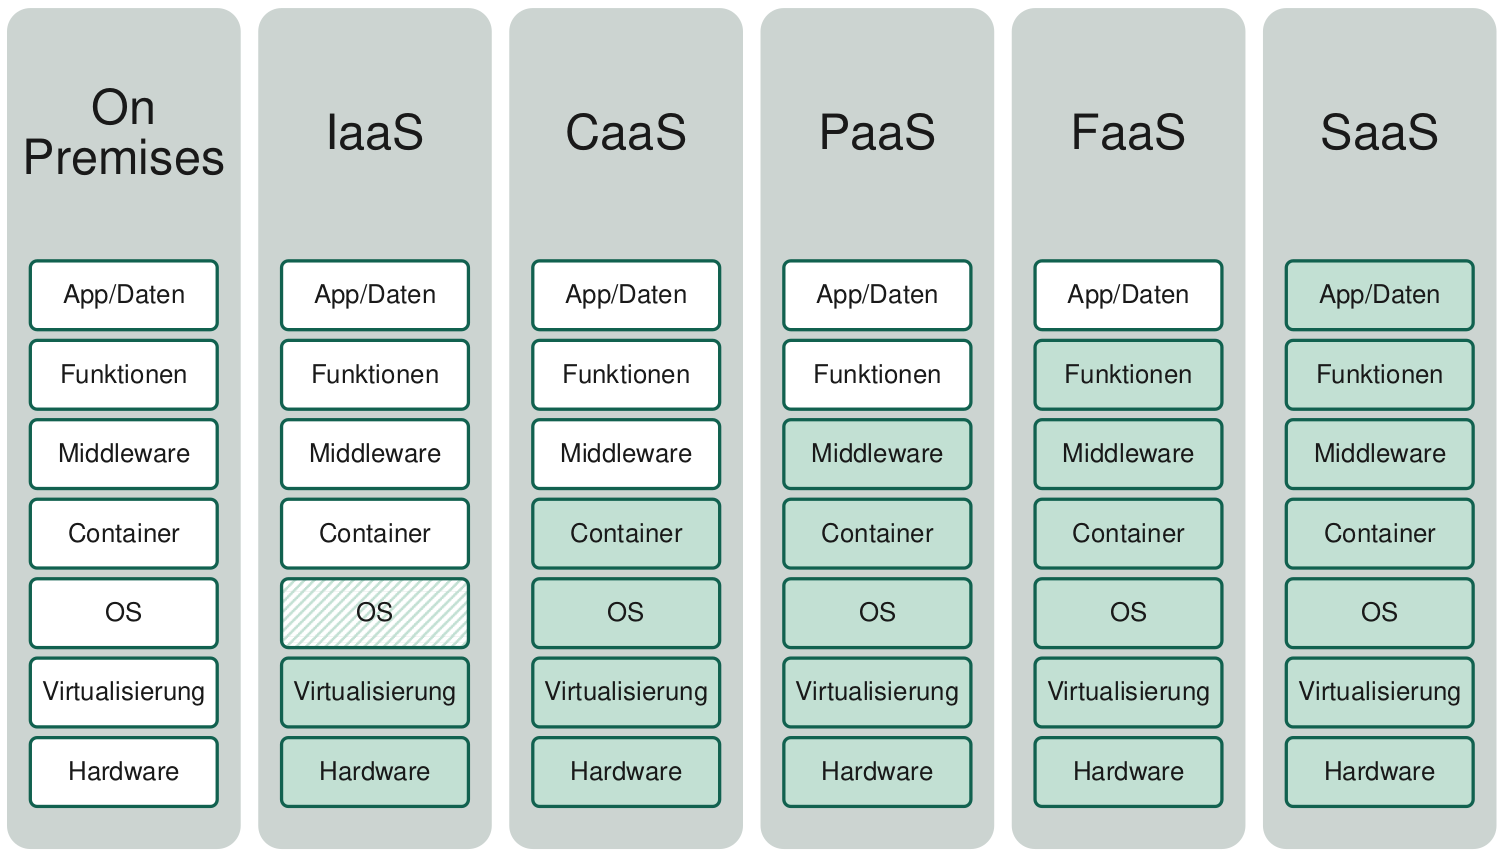
\includegraphics[width=\linewidth]{introduction2-cloud-service-classes.png}

Weiss $\rightarrow$ übernimmt der Kunde die Verantwortung
Grün $\rightarrow$ stellt der Cloud-Anbieter zur Verfügung

\begin{itemize}
    \item \textcolor{blue}{IaaS} Infrastructure as a Service, Skalierbare VM (virtuelle Maschinen), Cloud-Anbieter stellt virtuelle Maschinen mit frei konfigurierbarer Kapazität zur Verfügung
    \item \textcolor{blue}{CaaS} Container as a Service, Für die Installation von SCS, wie z.B. Microservices stellt der Cloud-Betreiber Container im Rahmen von Docker bzw. Kubernetes zur Verfügung.
    \item \textcolor{blue}{PaaS} Platform as a Service, Cloud-Anbieter stellt unterschiedliche Middleware, wie Runtime-Umgebung, Frameworks und ähnliches zur Verfügung (Bsp. Serverless Azure Web-Anwendung). Einzelne Dienste aus der Cloud
    \item \textcolor{blue}{FaaS} Function as a Service, Für serverlose Applikationen bedienen sich die Entwickler einer Fülle von Einzel-Funktionen. Bietet höchste Fle-
    xibilität und Skalierbarkeit. Das Beispielsweise AWS Lambda, Azure Functions, Google Cloud Functions
    \item \textcolor{blue}{SaaS} Software as a Service, Gesamte Applikation wie z.B. CRM (Customer Relationship Management) wird vollständig und betriebsbereit zur Verfügung gestellt.
\end{itemize}

\subsubsection{Prüfungsfragen}

\begin{itemize}
    \item Zeichnen Sie das Client-Server Modell mit einem UML Komponentendiagramm auf und zeigen Sie die Schnittstelle sowie die Interkation auf \\
    \textcolor{blue}{Antwort}
    \item Nennen Sie vier konkrete Eigenschaften von SCS \\
    \textcolor{blue}{lose Kopplung, wenige Abhängigkeiten, hohe Kohäsion, wohldefinierte Aufgabe}
    \item Welche Schichten enthalten der Web Tier? Welche Funktionen übernehmen diese und welchen Gesamtzweck hat der Web Tier? \\
    \textcolor{blue}{Prasentation Tier (innerhalb Applikation) und Service Tier (ausserhalb Applikation). Bietet Schnittstelle zum Server an}
    \item Welche Schichten muss eine Applikation aufweisen, damit sie SOA-enabled ist? \\
    \textcolor{blue}{API-Gateway, Web Service Access Tier mit Proxy-Komponente}
\end{itemize}

        \vfill\null
        \columnbreak
        \subsection{Flexible Architekturen (Microservices)}

\subsubsection{Modelle}

\textbf{Monolith}

Nachteile
\begin{itemize}
    \item Einheitlicher langfristig einzusetzender Technologiestack
    \item \textcolor{blue}{erheblichen Koordinationsaufwand} Änderungen in der Architektur benötigen das Einverständnis bzw. Information aller, unter den Entwicklungsteams bei grosser fachlicher Breite für eine Applikation (z.B. ERP, CRM usw.), sowie der zentralen Stellen für das Deployment und Betrieb von Software
    \item Viele \textcolor{blue}{gegenseitige Abhängigkeiten} erschweren die Weiterentwicklung.
    \item \textcolor{blue}{Testing} betrifft alle Schichten und ganze Breite der Funktionalität. Daraus erfolgen Releasezyklen von mehreren Monaten
    \item Serverseitige \textcolor{blue}{Änderungen} und Erweiterungen für neue Technologien, wie z.B. Augmented Reality, IoT usw. stossen auf erhebliche Schwierigkeiten
    \item \textcolor{blue}{Deployment} ist komplex und kann nur in grösseren zeitlichen Abständen vorgenommen werden
    \item \textcolor{blue}{Migration} auf eine neue Technologie ist äussert
    aufwendig
\end{itemize}
\vspace{10pt}
\textbf{Self-Contained System (SCS) Microservices}

SCS nimmt eine vertikale Aufteilung der Applikation in fachliche Funktionen vor, wie z.B. Artikelservice, Kundenservice, Bestellservice usw. Enthalten alle notwendigen Schichten analog der Mehrschichtenarchitektur (Applikation wird in mehrere unabhängige Systeme aufgeteilt), jedes SCS ist eine unabhängige Web-Applikation mit eigenem GUI, Kommunikation zwischen SCS erfolgt per default asynchron, jedes SCS hat eigenständige Logik und Daten \\

Vorteile
\begin{itemize}
    \item lose Kopplung
    \item wenige Abhängigkeiten
    \item hohe Kohäsion
    \item wohldefinierte Aufgabe
\end{itemize}
\vspace{10pt}
\textbf{Microservice}

1 SCS kann aus 1-x Microservices bestehen, Bildet eine eigenständige fachlich klar fokussierte, eingegrenzten (Teil)funktion einer Applikation ab, Ihm steht ein eigener Ausführungscontainer/Laufzeitumgebung (Docker) zur Verfügung, Der Zugriff erfolgt über eine klar definierte synchrone und/oder asynchrone Schnittstelle \\

Vorteile
\begin{itemize}
    \item \textcolor{blue}{Klare fachliche Abgrenzung} mit sauberer Trennung der Zuständigkeiten je Service
    \item \textcolor{blue}{Lose Kopplung, möglichst Stateless} Ermöglicht einfaches Auswechseln der Komponenten
    \item \textcolor{blue}{Hohe Skalierung und Fehlertoleranz} Es können mehrere Scrum-
    Teams parallel an unterschiedlichen Microservices entwickeln
    \item \textcolor{blue}{Hohe technische Unabhängigkeit} Jedes Team hat innerhalb der für die Unternehmung strategisch festgelegten Plattformen die Freiheit, die optimale Technologie zu wählen
    \item \textcolor{blue}{Hohe Resilienz (Robustheit)} da Störung einer Komponente
    die anderen nicht beeinflussen
    \item \textcolor{blue}{Hohe Automatisierung} im CI/CD im DevOps-Kontext: \\ 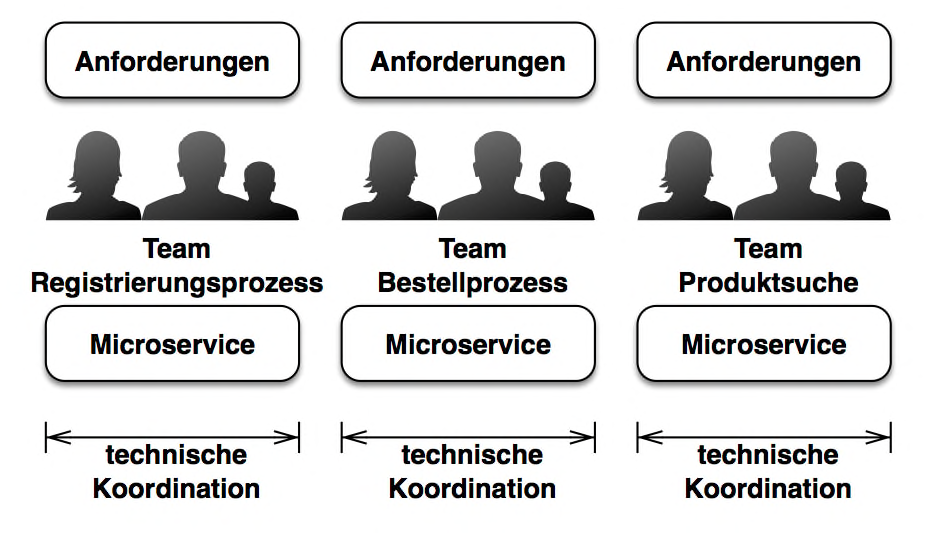
\includegraphics[width=\linewidth]{microservices-advantages.png}
\end{itemize}
\vspace{10pt}
Nachteile

\begin{itemize}
    \item Erhöhung der \textcolor{blue}{Gesamtkomplexität} durch die Zahl der Microservices
    \item Einsatz von \textcolor{blue}{unterschiedlichen Technologien} bedingt Erhalt des Knowhows $\rightarrow$ Verringert Flexibilität der Austauschbarkeit der Projektmitarbeiter
    \item \textcolor{blue}{Optimale Grösse} für Microservices muss gefunden werden (zu gross $\rightarrow$ Weiterentwicklung im gleichen Team kann nicht gewährleistet wer-
    den, zu klein $\rightarrow$ Komplexität der Interaktion und Abhängigkeiten steigen)
    \item \textcolor{blue}{Refactoring} das fachliche Teile von anderen Services herausschneidet, kann sehr aufwendig sein
    \item Lattenz beeinflusst die Performance negativ
\end{itemize}

\subsubsection{Domain Driven Design (DDD)}

Ist eine Vorgehensweise, um in komplexen Applikationen im strategischen Design die Fachdomänen mit klaren Kontextgrenzen herauszufinden und im taktischen Design im Detail zu spezifizieren.

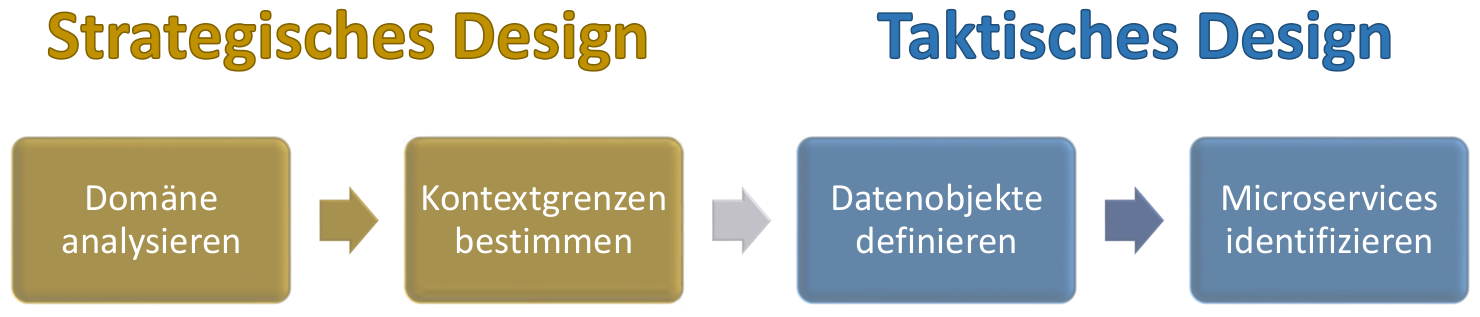
\includegraphics[width=\linewidth]{microservices-ddd.png} \\

\textbf{Strategisches Design}

\begin{itemize}
    \item Domäne analysieren
    \item Bounded Contexts festlegen (Fachlich klar abgegrenzter Kontext)
    \item Ubiquitous Language (Begriffe in einem Bounded Context) erarbeiten
    \item Context Map erstellen
\end{itemize}
\vspace{10pt}
\textbf{Taktisches Design}

\begin{itemize}
    \item (OO)-Entwurf in einem Bounded Context vornehmen
    \item Domain Events herausfinden
\end{itemize}
\vfill\null
\columnbreak
\subsubsection{Makroarchitektur}

\textbf{Persistenz}

Microservices haben eigene DB

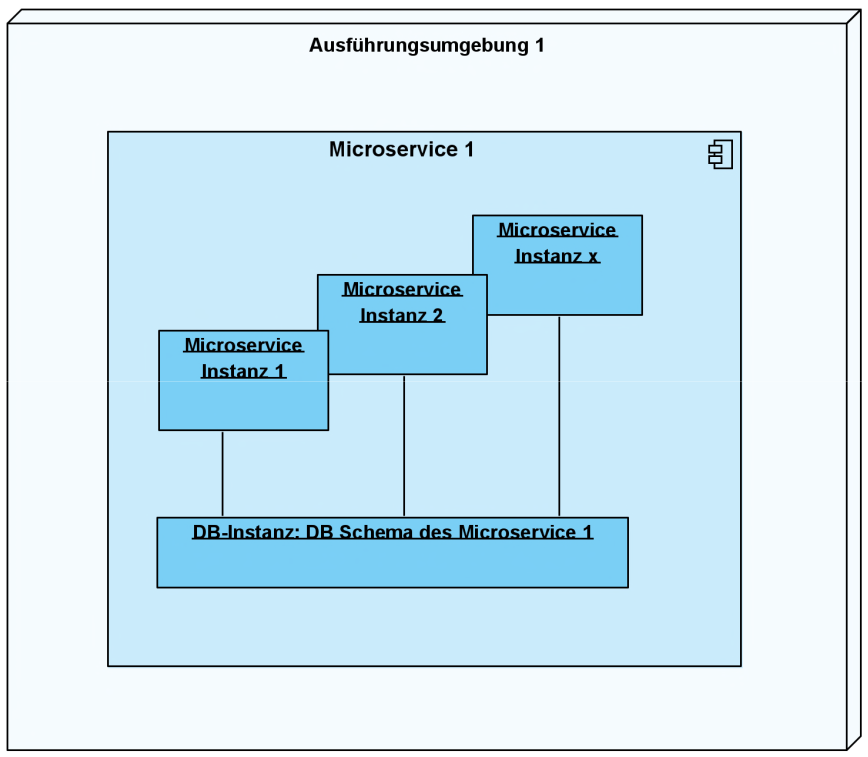
\includegraphics[width=0.8\linewidth]{microservices-persistence-1.png} \\

Zentraler DB-Service

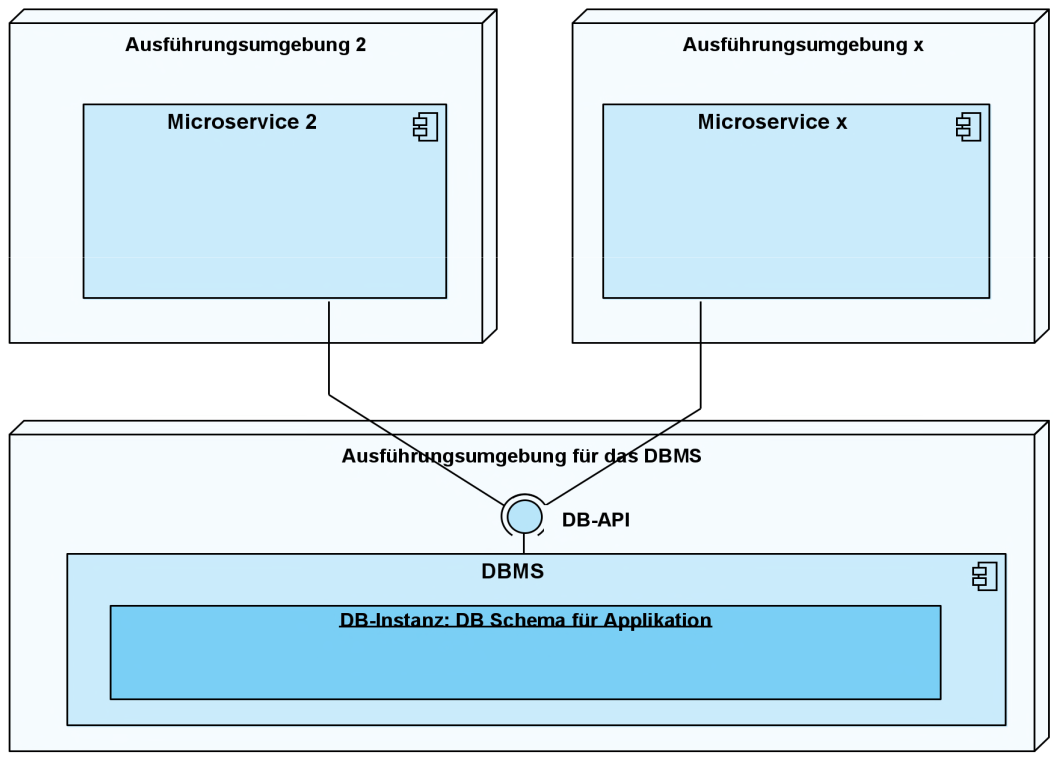
\includegraphics[width=0.8\linewidth]{microservices-persistence-2.png} \\

\textbf{Referenz-Makroarchitekturen}

\begin{itemize}
    \item \textcolor{blue}{API-Gateway} Bietet geeignete Web Service für Service Consumer an. Zugrunde liegende Middleware übernimmt Aufgaben wie Authentisierung, Atuorisierung, SSL/TLS-Endpoint, Web App Firewall (WAF), Logging, Service-
        Registry, Skalierung/Load-Balancing, Caching usw.
    \item \textcolor{blue}{Docker Host} Bietet für jeden Microservice Container an
    \item \textcolor{blue}{MOM} Messaging zwischen den Microservices erfolgt asynchron über einen Message Broker
    \item \textcolor{blue}{Shared Services} Microservices die allen anderen Microservices zur Verfügung stehen. Übernehmen meist Querschnittsfunktionen und können, eigene Persistenz enthalten
    \item \textcolor{blue}{Proxy Service} Übernimmt Kommunikation zu den applikationsexternen Service Provider und enthält meist eigenen Cache-Speicher
\end{itemize}
\vfill\null
\columnbreak
Full Server-Stack Microservices (Microservices als SCS)

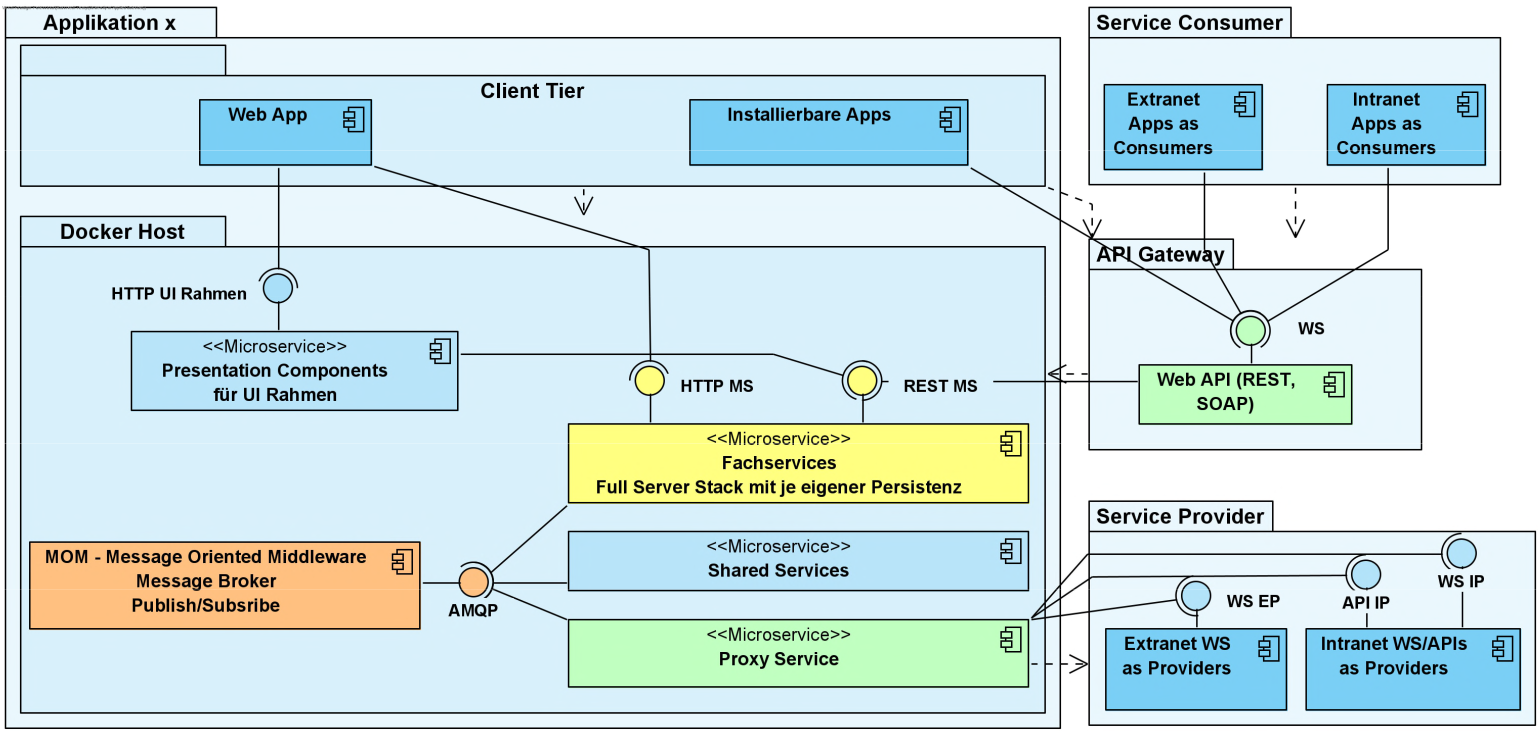
\includegraphics[width=\linewidth]{microservices-scs.png}

\begin{itemize}
    \item \textcolor{blue}{Client} UI Rahmen App und separate installierbare Client App (z.B. Mobile App)
    \item \textcolor{blue}{Persistenz} jeder Microservice hat eigene Persistenz
    \item \textcolor{blue}{Kommunikation} asynchrones Messaging über die MOM (Message Oriented Middleware), Zugriff auf Service Provider über einen zentralen proxy Microservice
\end{itemize}
\vspace{10pt}

\textbf{Beispiele}

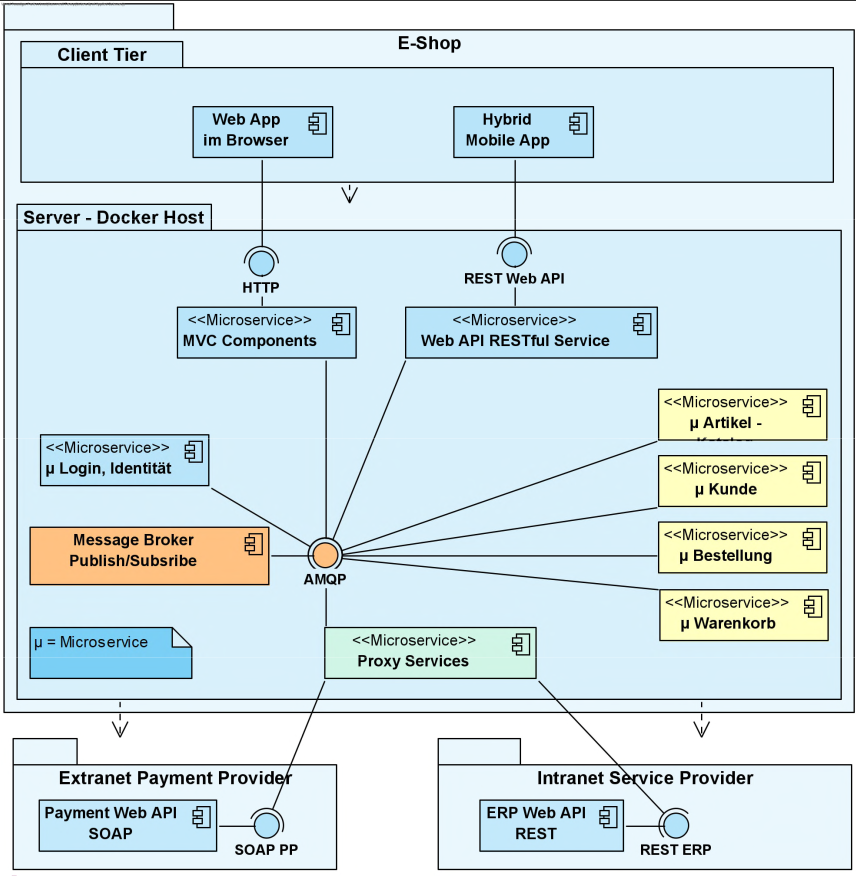
\includegraphics[width=\linewidth]{microservices-example.png}

\begin{itemize}
    \item \textcolor{blue}{API-Gateway} Da keine applikationsexterne Consumer vorgesehen sind, wird dieser weggelassen.
    \item \textcolor{blue}{Client Applikation} 2 Client Applikationen sind vorgesehen
    \begin{itemize}
        \item \textcolor{blue}{Web App} Kommuniziert mit MVC Components z.B. ASP.NET MVC
        \item \textcolor{blue}{Hybrid Mobile App} Kommuniziert mit Server über REST
    \end{itemize}
    \item \textcolor{blue}{Messaging} erfolgt asynchron über Message Broker mit dem AMQP-Protokoll
    \item \textcolor{blue}{Fachlogik} Ist auf 4 Microservices aufgeteilt. Jeder Microservice verfügt über eigene Persistenz.
    \item \textcolor{blue}{? Login, Identität} ist Querschnitts-Microservice, der Login-Daten persistent hält
    \item \textcolor{blue}{Proxy Services} Für die Kommunikation zu den beiden applikationsexternen Service Provider existieren je eine eigene Proxy-Komponente, welche in einem Microservice vereint sind
\end{itemize}
\vspace{10pt}
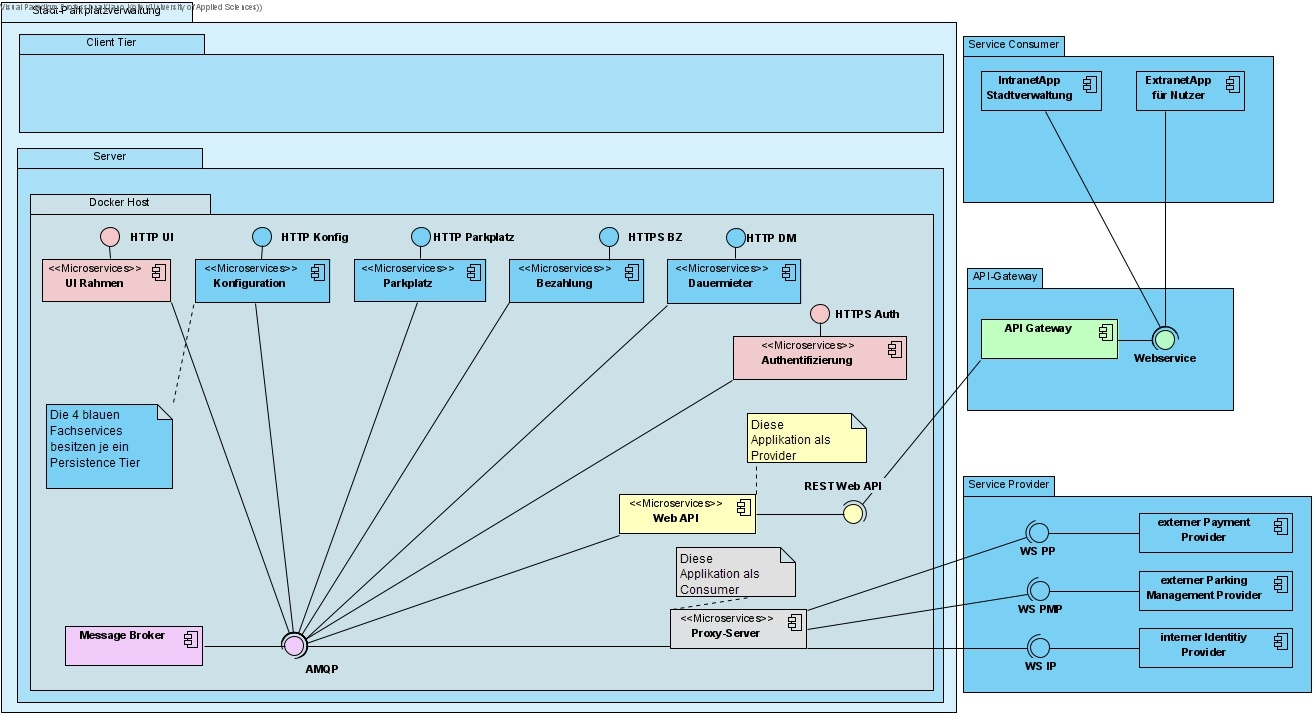
\includegraphics[width=\linewidth]{microservices-example-cars.png}

\subsubsection{Microarchitektur}

Jeder Mikroservices hat sein eigener Technologie-Stack, Dieser ist auf das zu beschränken, was benötigt wird

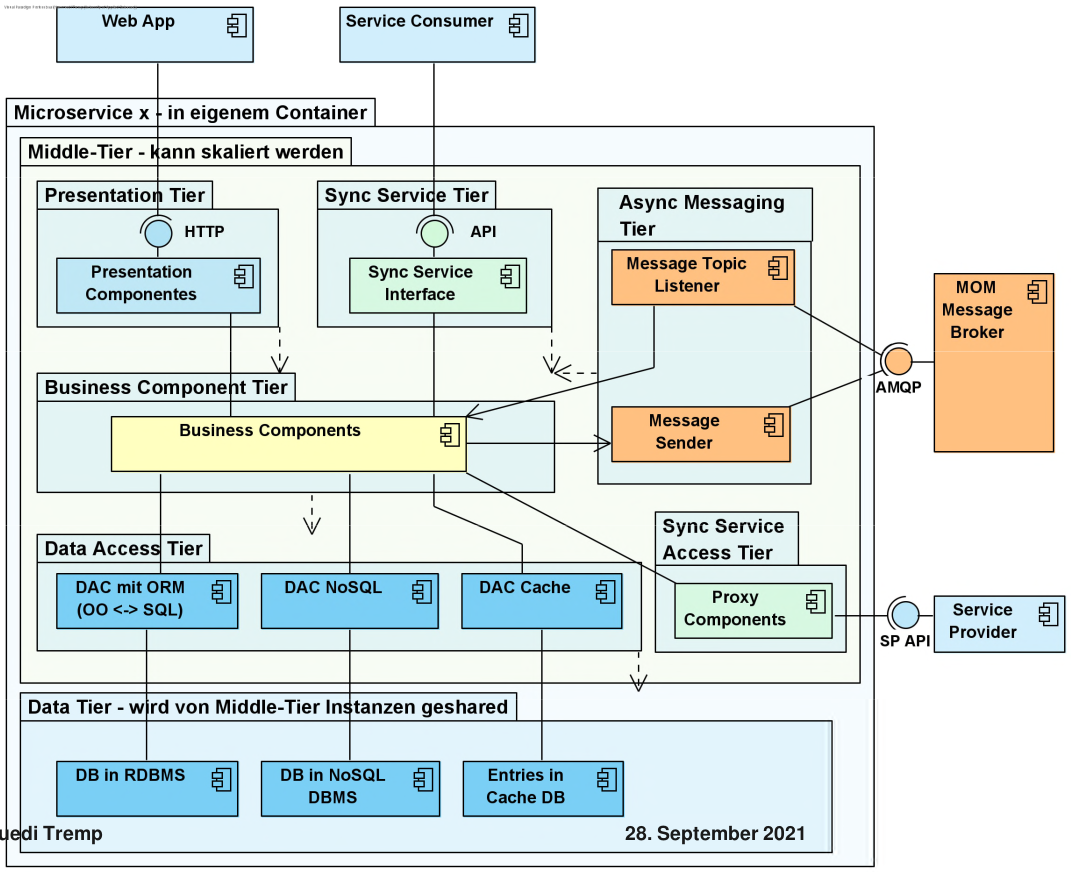
\includegraphics[width=\linewidth]{microservices-micro-architecture.png}

\subsubsection{Containerisierung}

mit Docker

\begin{itemize}
    \item Lifecycle-Management von Container: Planung, Konfiguration, Registrierung
    \item Provisionierung und Bereitstellung der Container
    \item Zuweisung der Ressourcen
    \item Skalierung der Container und Load-Balancer
    \item Sichern der Interaktion zwischen den Containern
    \item Monitoring
\end{itemize}

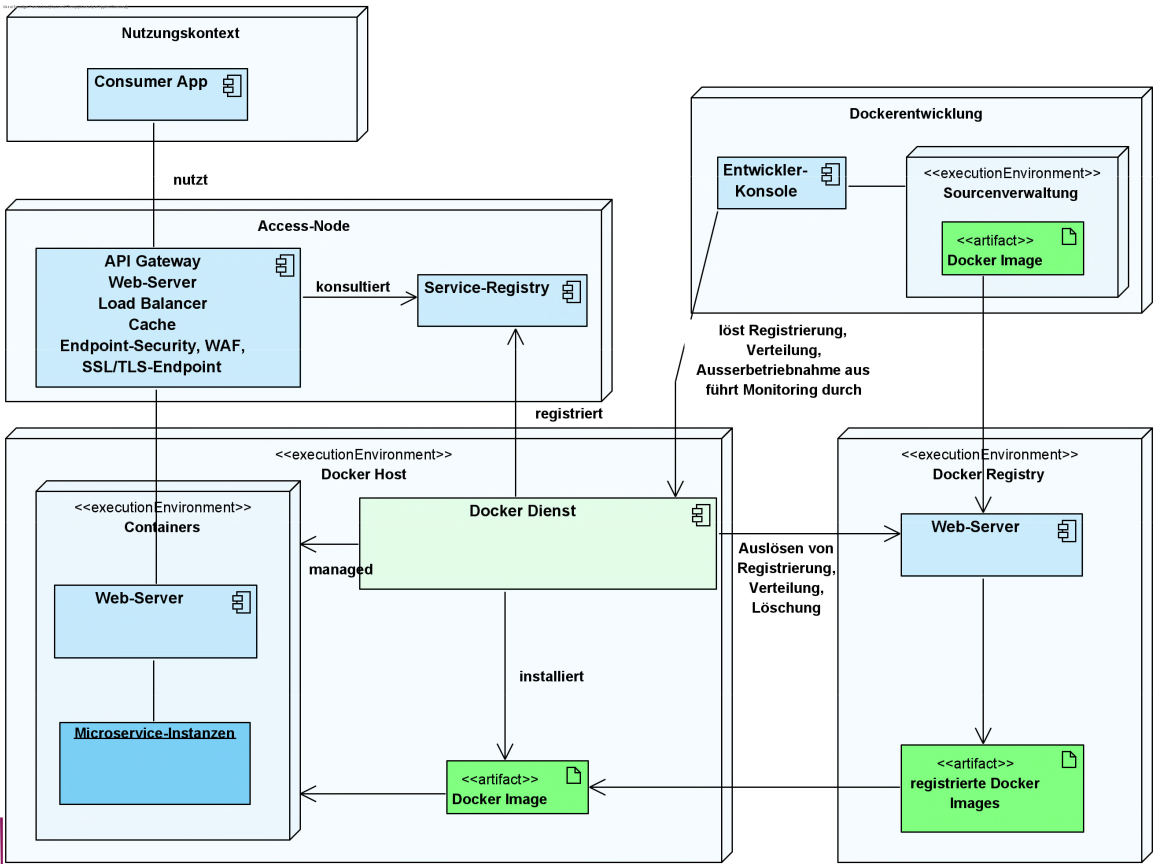
\includegraphics[width=\linewidth]{microservices-docker.png}

\columnbreak
\subsubsection{Prüfungsfragen}

\begin{itemize}
    \item Was spricht gegen ein applikationsweites kanonisches(gemeinsames) Datenmodell im Umfeld von Microservices? \\
    \textcolor{blue}{Erhaltung der Datenkonsistenz}
    \item Modellieren Sie eine Makro-Softwarearchitektur mit folgenden Elementen: Mobile-Client-App, API-Gateway, 3 Microservies, 1 Proxy-Microservice, 1 Extranet Web Service Provider \\
    \textcolor{blue}{Antwort}
    \item Inwiefern unterscheidet sich ein Container von einer VM? \\
    \textcolor{blue}{VM hat OS und Container nicht}
    \item Sie wollen hunderte von Ihren Microservices flexibel und sicher betreiben, CI/CD automatisieren, anhand des Traffics optimal skalieren und überwachen. Welche Art Software benötigen Sie dafür? Für welche konkrete Software entscheiden Sie sich? Geben Sie mindestens zwei Gute Gründe für Ihren Entscheid. \\
    \textcolor{blue}{Container-Orchestrierung $\rightarrow$ Kubernetes, weil es gut mit Docker harmonisiert}
\end{itemize}



        \vfill\null
        \columnbreak
        \subsection{Clientseitige Architektur}

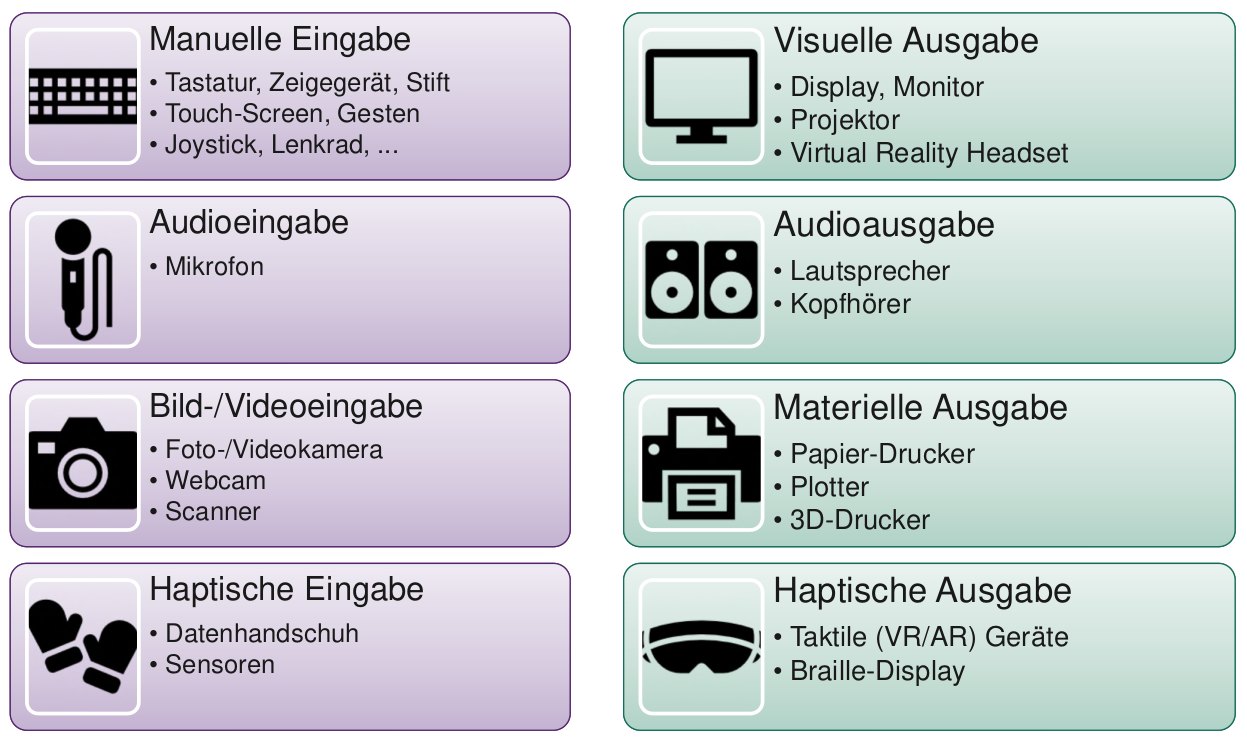
\includegraphics[width=\linewidth]{clients-hci.png}

\begin{itemize}
    \item \textcolor{blue}{Desktop Device}
    \item \textcolor{blue}{Mobile Device} Tablet, Notebook, Wearable Devices, Mobile Phone
    \item \textcolor{blue}{IoT Device} physischen Kontext (Cyber-Modell, Applikation, Analytik)
    \item \textcolor{blue}{Virtueller Device} Client zeigt nur Bild an, Verarbeitung läuft auf dem Server
\end{itemize}

\subsubsection{Client OS}

\begin{itemize}
    \item Windows
    \item Apple
    \item Linux
    \item Android
\end{itemize}

\subsubsection{Client App Technologien}

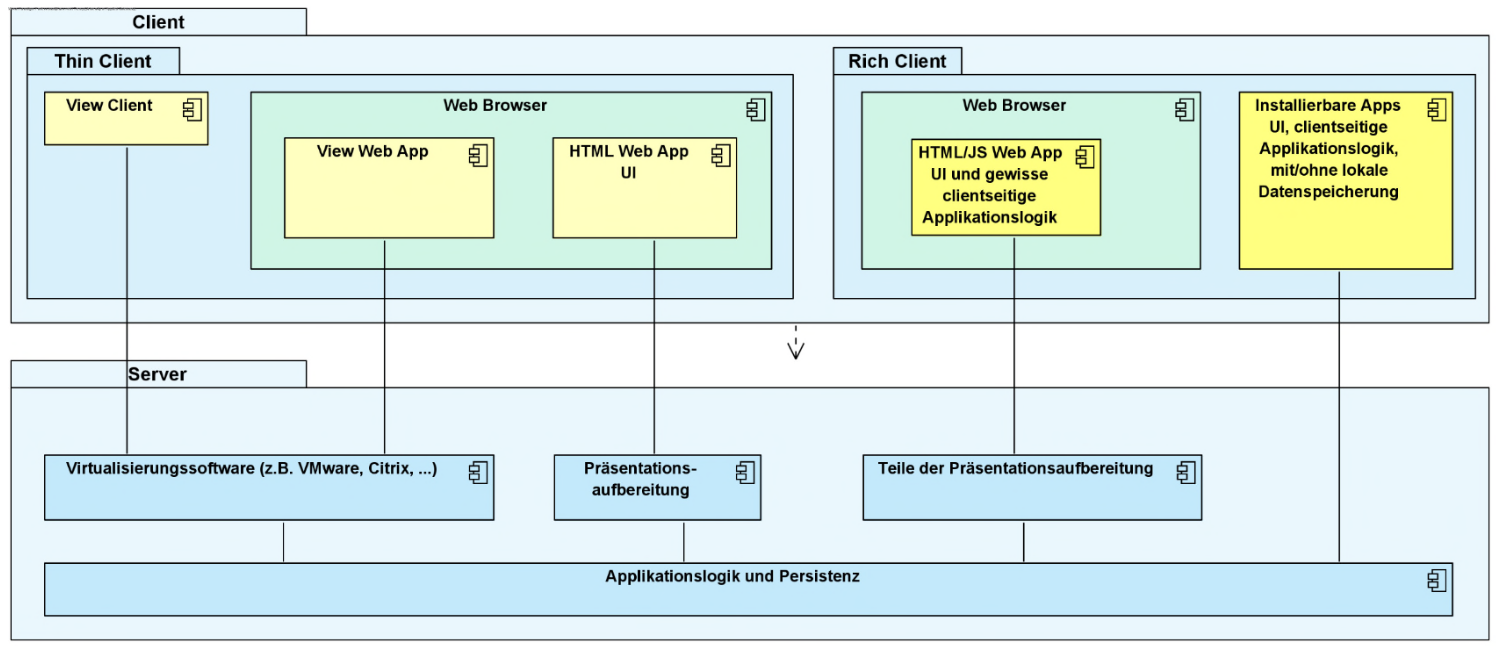
\includegraphics[width=\linewidth]{clients-devices.png} \\

\textbf{Thin Clients}

Virtuelle Desktops (VMware, Citrix), Werden im Webbrowser oder in View Clients betrieben \\

\textbf{Rich Client}

Klassische Desktop Apps, Haben meist nebst Applikationslogik, lokale Datenhaltung \\

\vfill\null
\columnbreak
\subsubsection{Location-L}

Location Based Services (LBS)

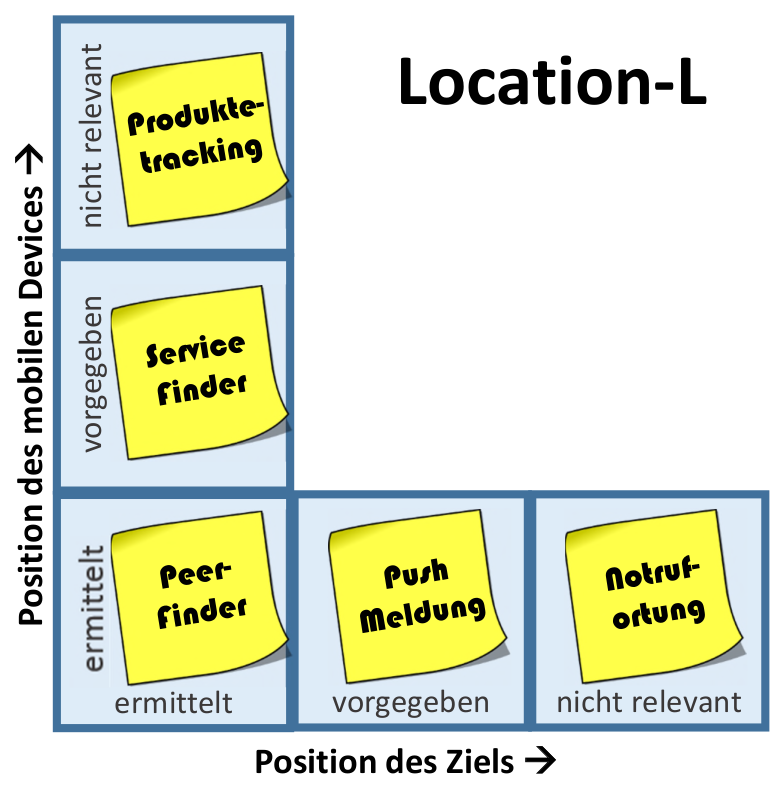
\includegraphics[width=0.7\linewidth]{clients-l.png}

Ein Standort muss mindestens ermittelt werden!

\subsubsection{Architekturmuster/Entwurfsmuster}

\textbf{Model View Controller (MVC)}

ASP.NET oder JSF

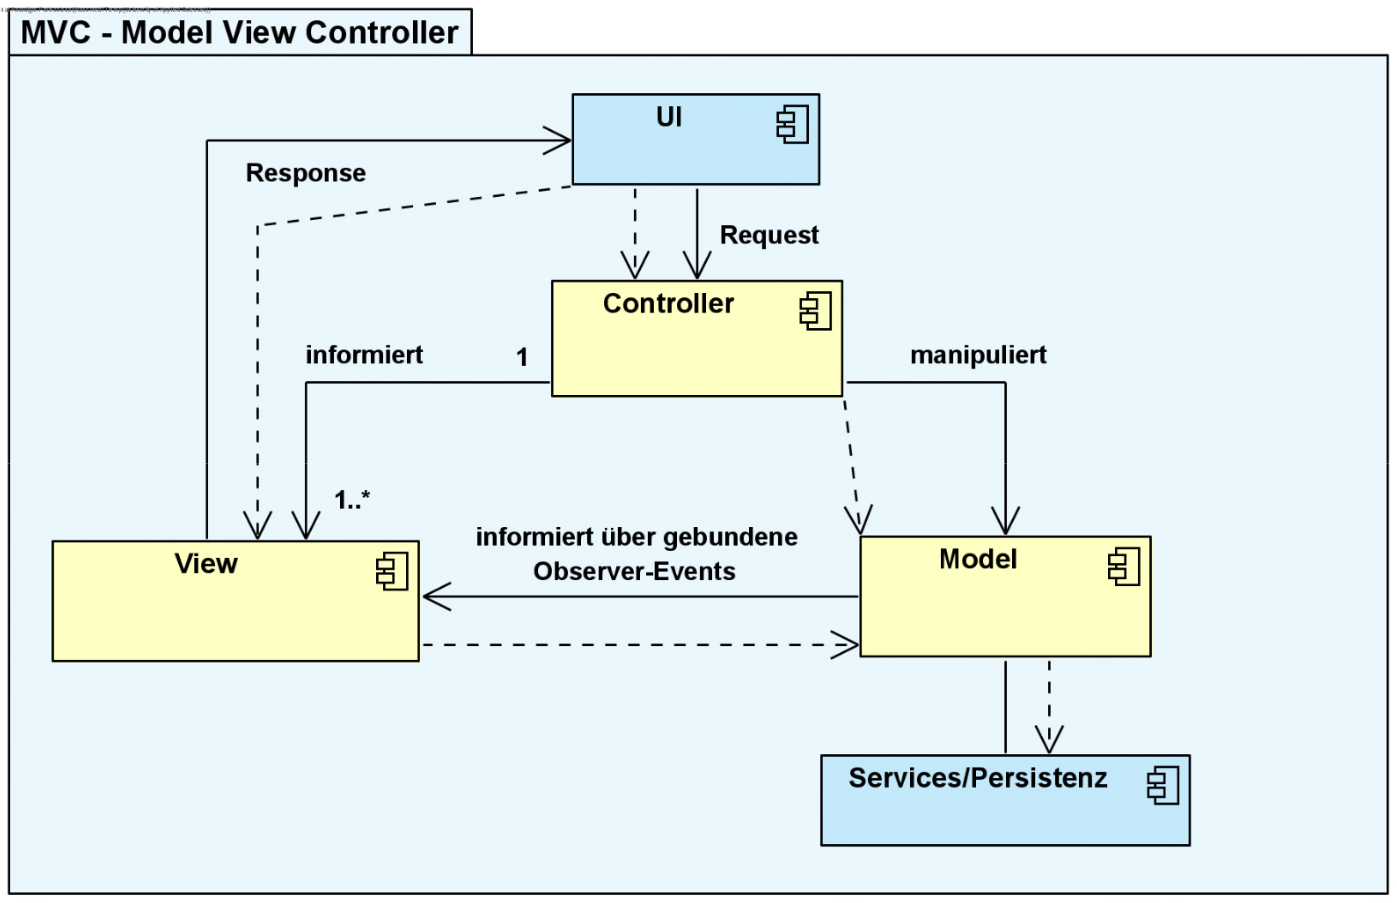
\includegraphics[width=\linewidth]{clients-mvc.png} \\


\textbf{Model View Presenter (MVP)}

bessere Testbarkeit der Komponenten und vollständiges Entkoppeln der View von dem Model. (Windows Forms)

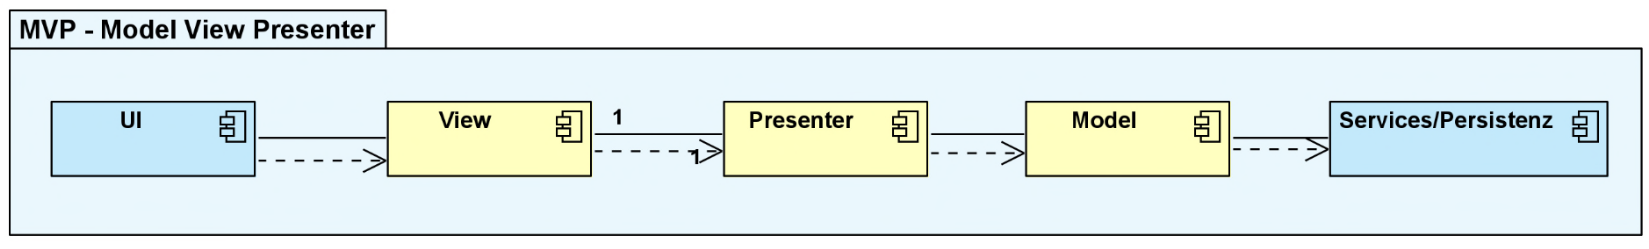
\includegraphics[width=\linewidth]{clients-mvp.png} \\

\textbf{Model View View-Model (MVVM)}

Web App

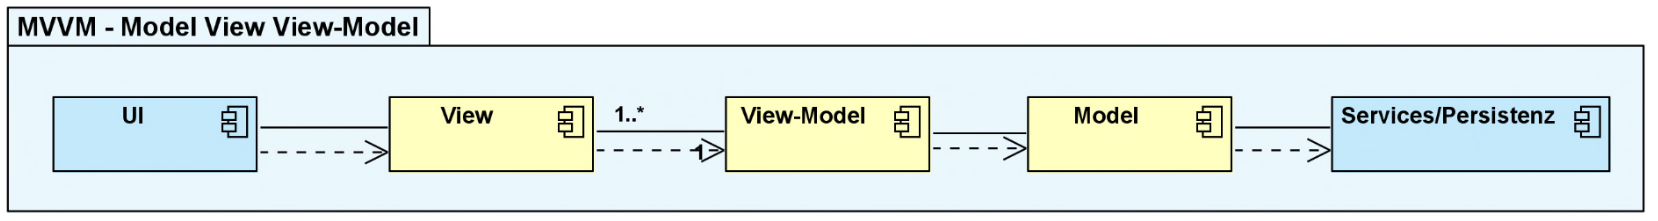
\includegraphics[width=\linewidth]{clients-mvvm.png} \\

\vfill\null
\columnbreak

\subsubsection{Programmiersprachtypen}

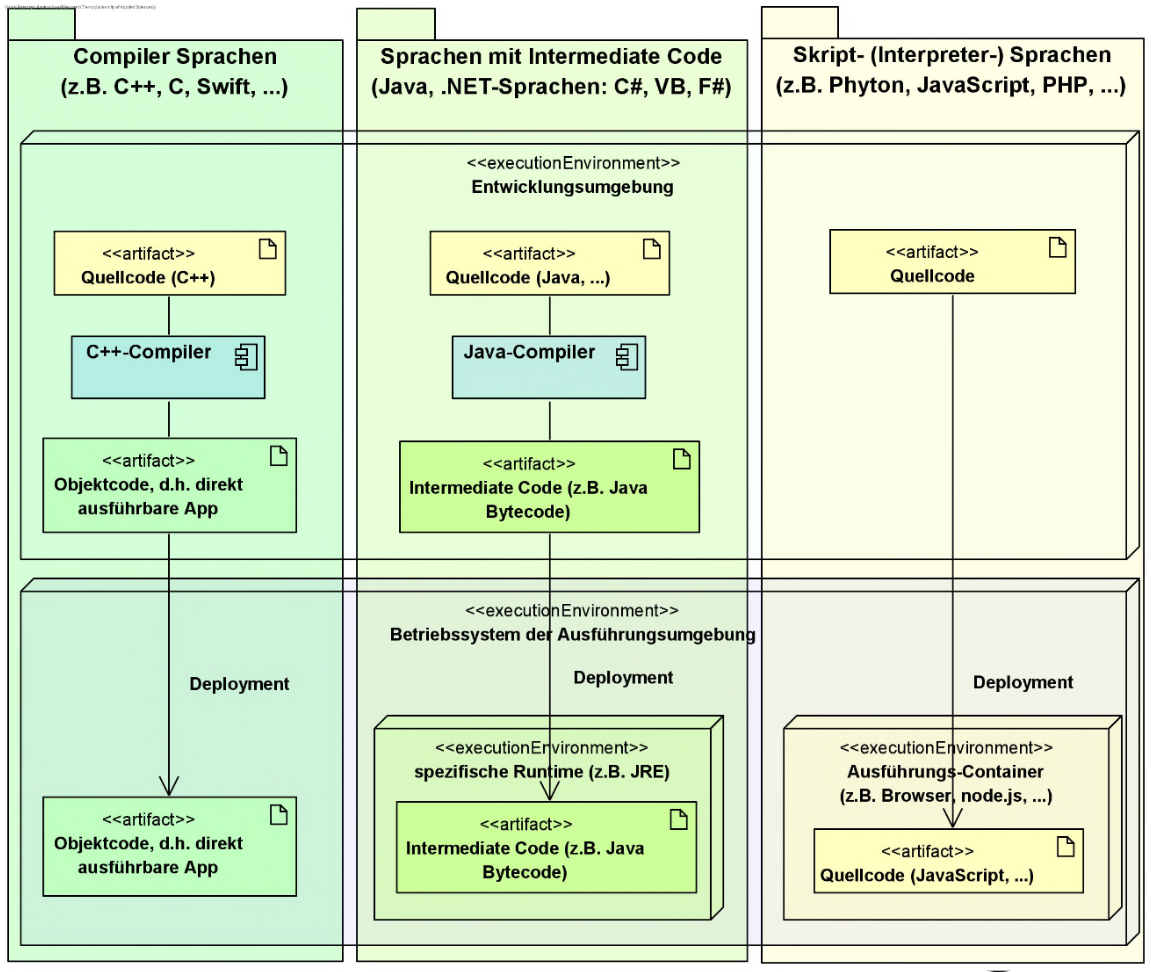
\includegraphics[width=\linewidth]{clients-programming-lang-types.png} \\

\subsubsection{Installable Client Apps}

Installable App

\textbf{Single Platform Apps} \\


\textbf{Cross Platform Apps}

\begin{itemize}
    \item Code kann gemeinsam genutzt werden
    \item Kostengünstiger
    \item Schneller Time-to-Market
\end{itemize}
\vspace{10pt}
\textbf{Multiplatform/Hybrid Apps}

Vorteile
\begin{itemize}
    \item Nutzen Devices voll aus
    \item Beste Performance
    \item UI sind voll Plattformkonform
\end{itemize}
\vspace{10pt}

Nachteile
\begin{itemize}
    \item Aufwändig
    \item Je Plattform ein eigenes Entwicklerteam
\end{itemize}

\subsubsection{Client WebApps}

Ausführung im Web Browser

\textbf{HTML5 mit/ohne JS} \\

\textbf{SPA}

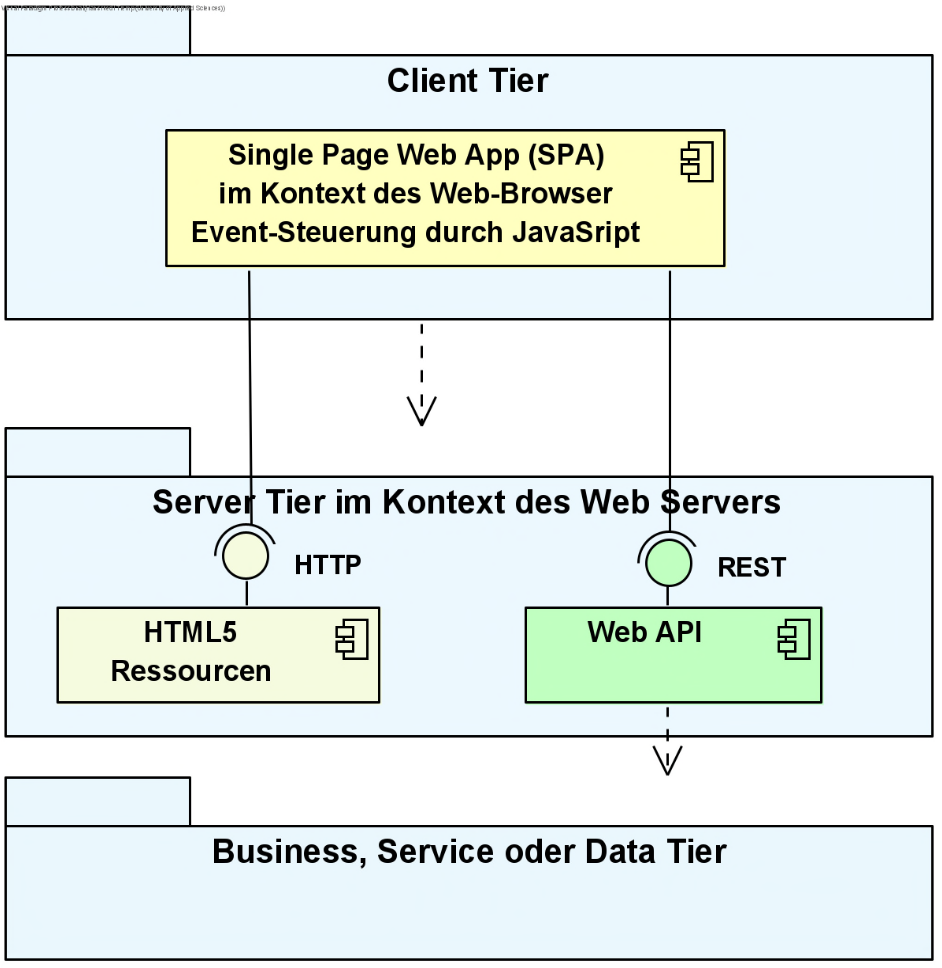
\includegraphics[width=0.7\linewidth]{clients-spa.png} \\

\textbf{PWA}

Webbrowser startet als unsichtbarer Container anhand der Informationen im Manifest, Requests erfolgen über Service Worker (Netzwerk vorhanden: Request beim Server vornehmen und Ergebnis im Cache aktualisieren, Netzwerk nicht vorhanden: Werte aus dem Cache auslesen)

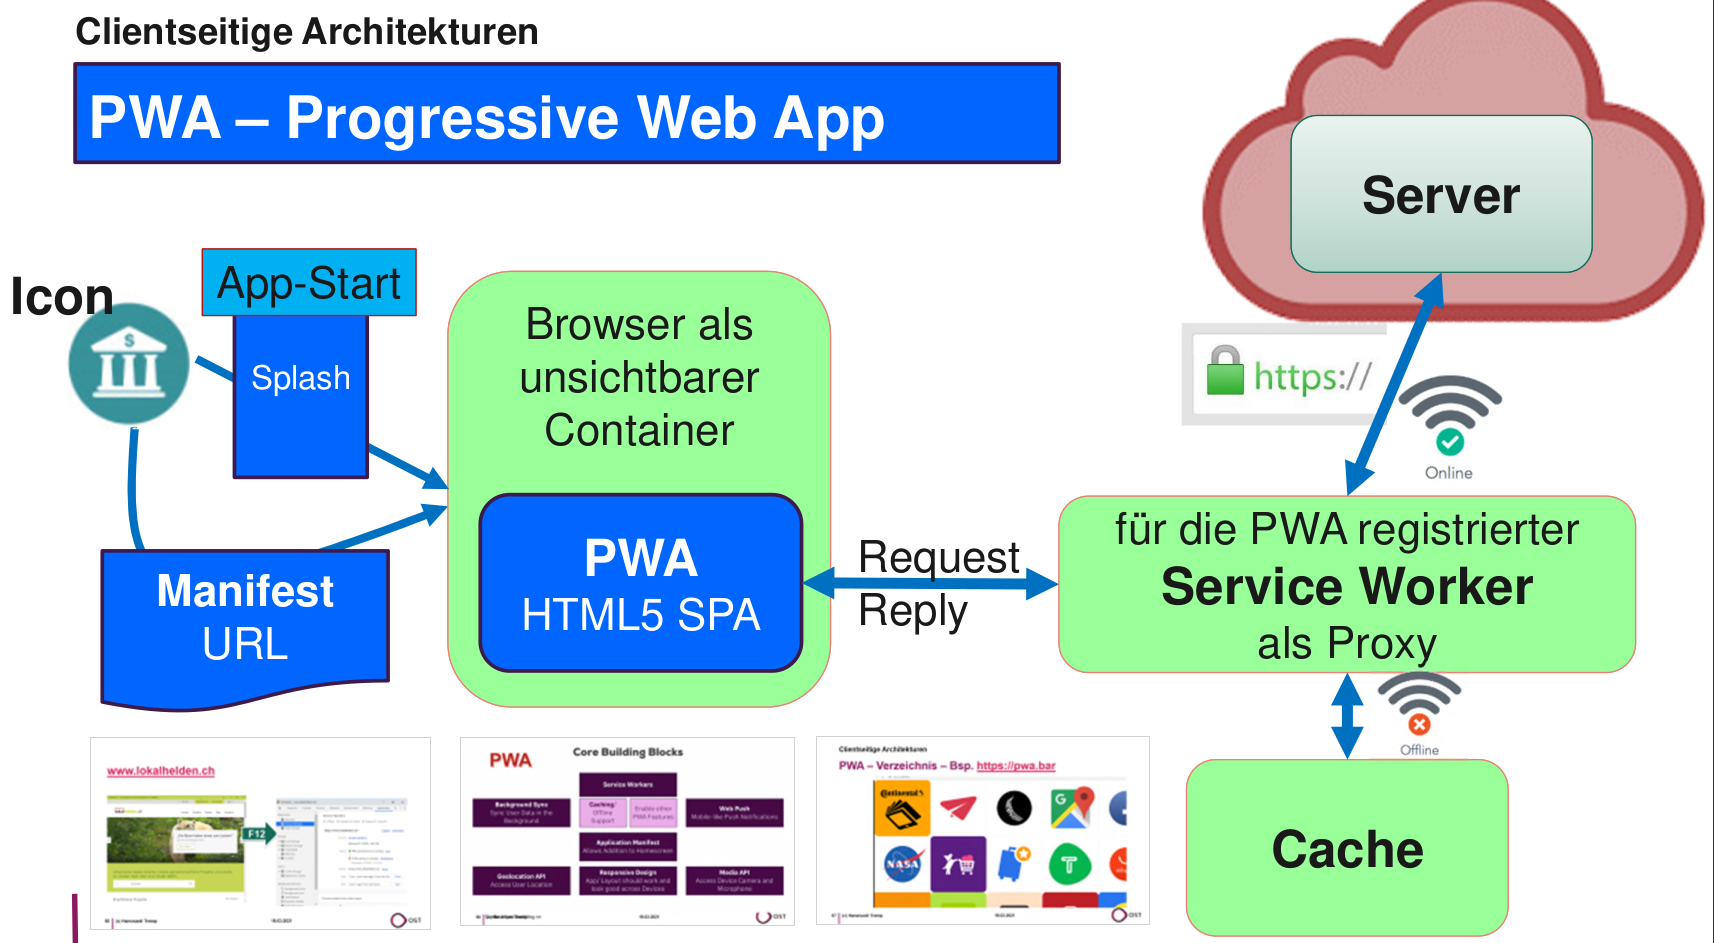
\includegraphics[width=\linewidth]{clients-pwa.png} \\

\textbf{Serverframework ASP.NET Core}

ASP – Active Server Page mit MVC Muster, Kestrel fungiert als Webserver

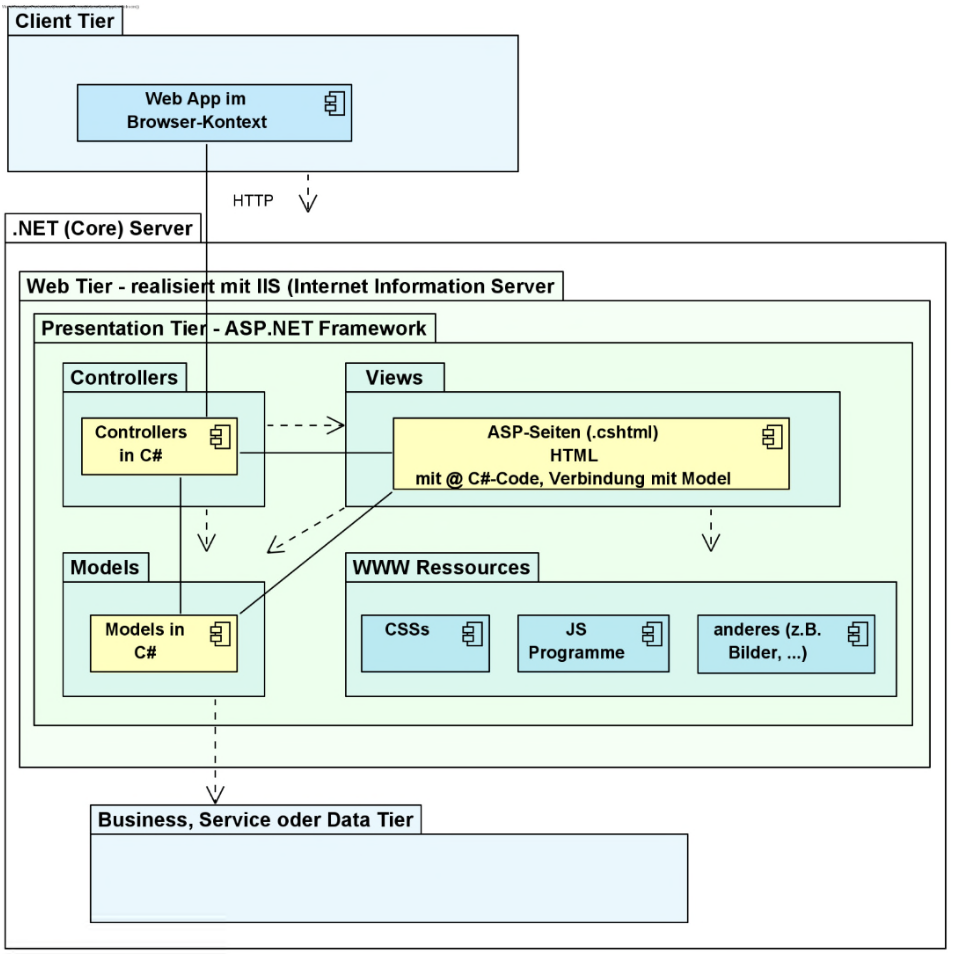
\includegraphics[width=\linewidth]{clients-asp.png} \\

\vfill\null
\columnbreak

\textbf{Serverframework Java EE}

JSF – Java Server Faces, zusätzlich Frameworks wie z.B. Spring usw., EJBs enthalten Business-Logik und die Connection zur DB

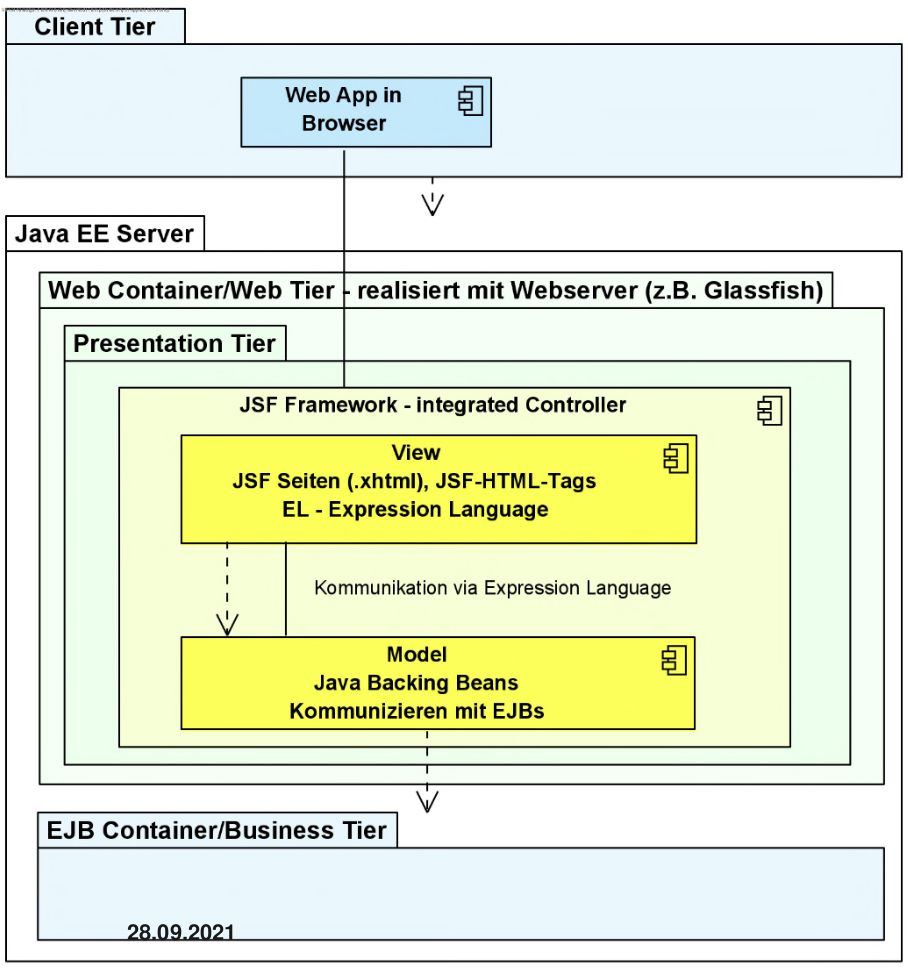
\includegraphics[width=\linewidth]{clients-java.png}

\subsubsection{Makroarchitektur}

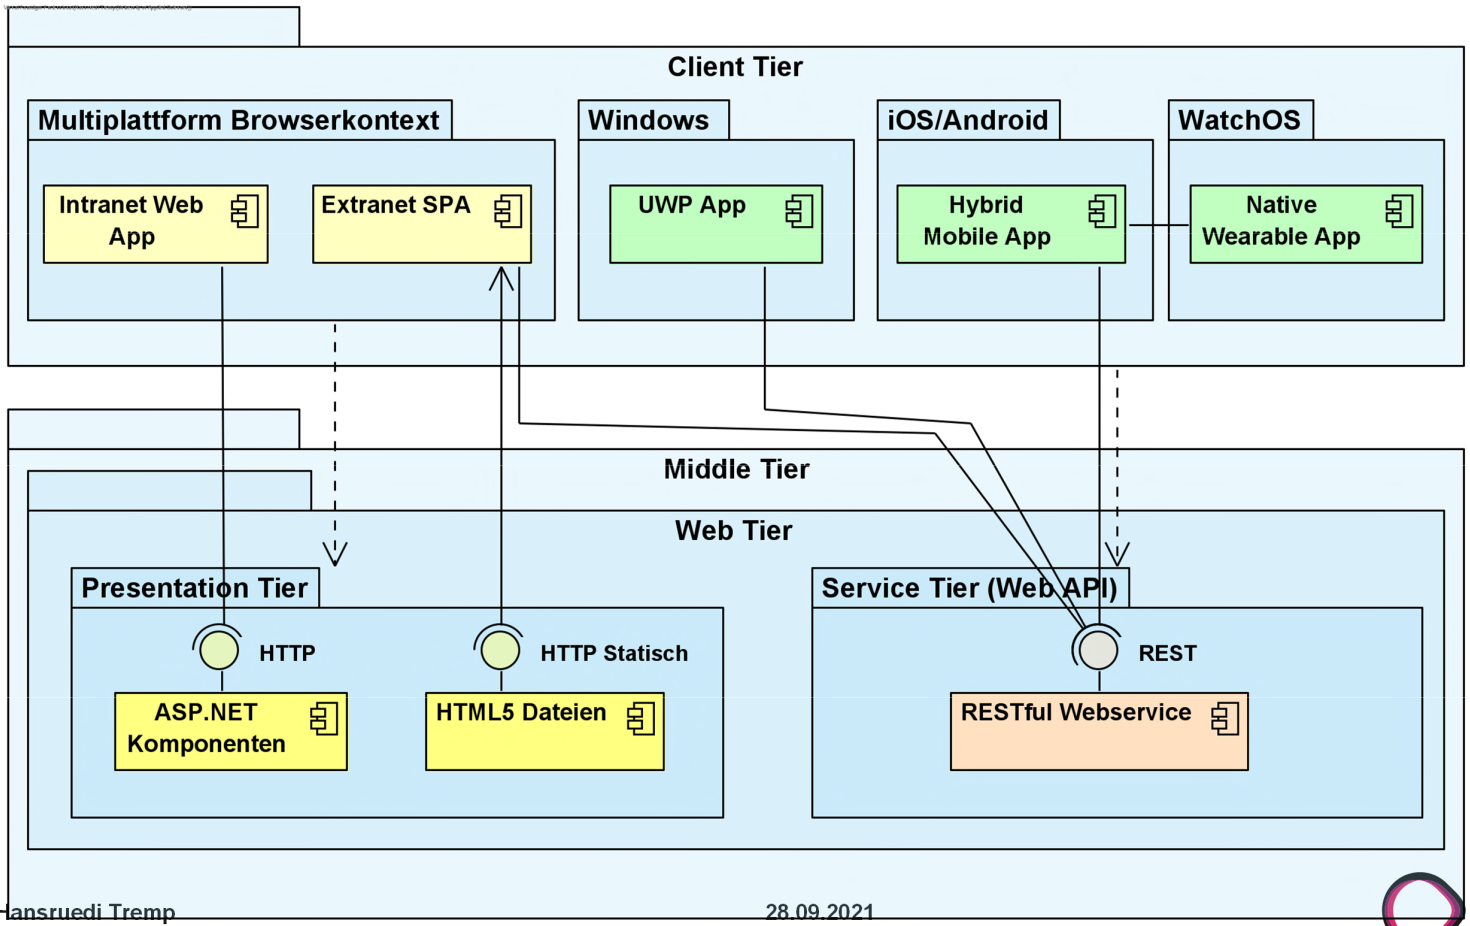
\includegraphics[width=\linewidth]{clients-macro-arch.png} \\

\vfill\null
\columnbreak

\textbf{UI}

Microservice hat sein eigenes UI

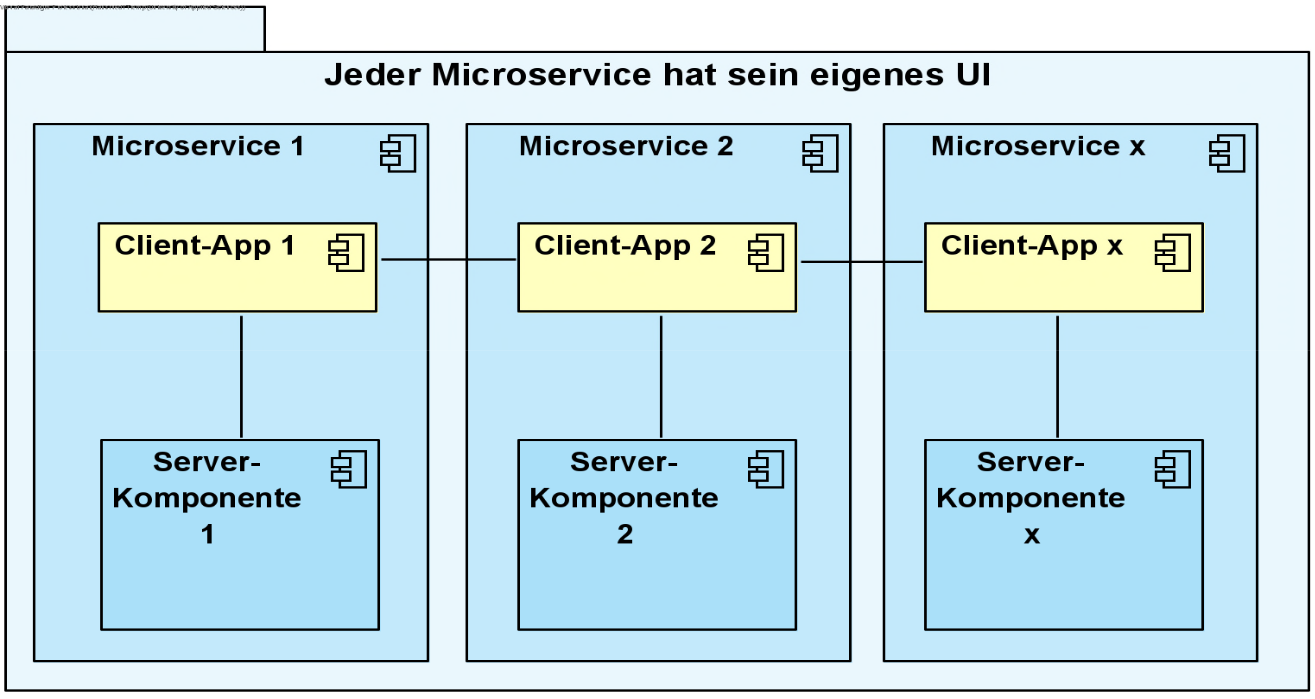
\includegraphics[width=0.8\linewidth]{microservices-ui-1.png} \\

Microservice gibt spezifischen Anteil zu UI Rahmen

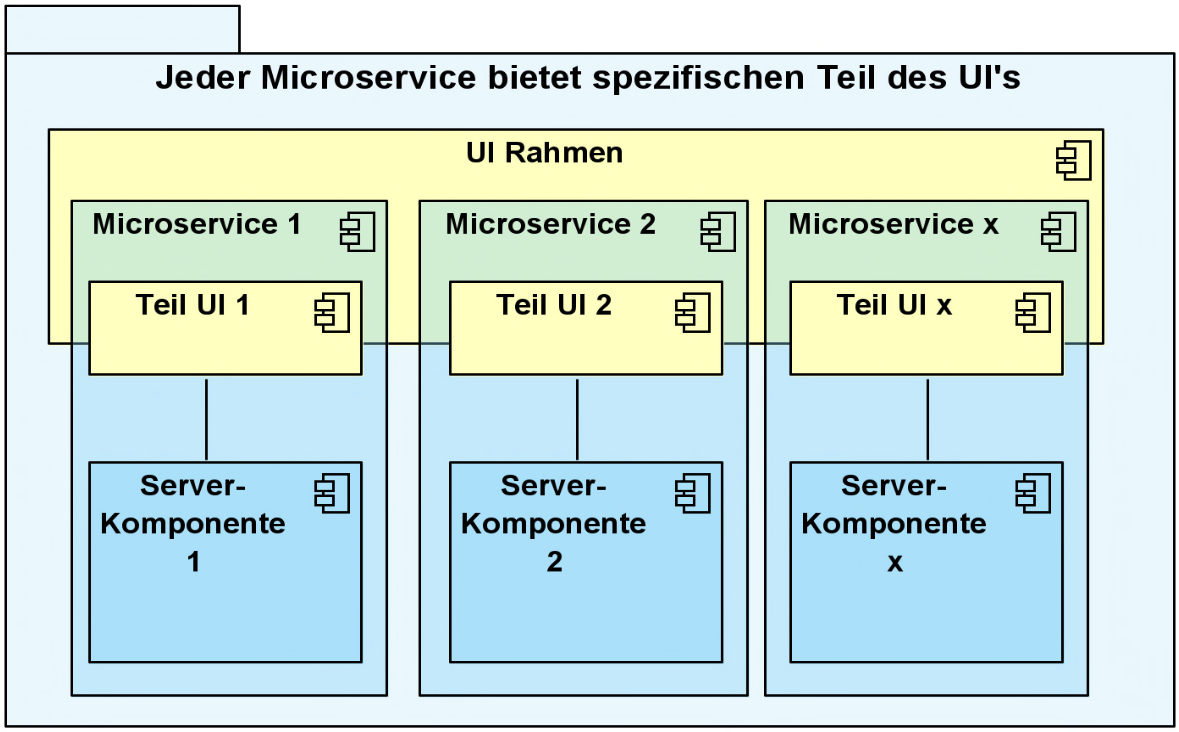
\includegraphics[width=0.8\linewidth]{microservices-ui-2.png} \\

Microservies haben kein UI sondern nur Service-Schnittstelle, dieses wird stattdessen realisiert durch UI Full Client

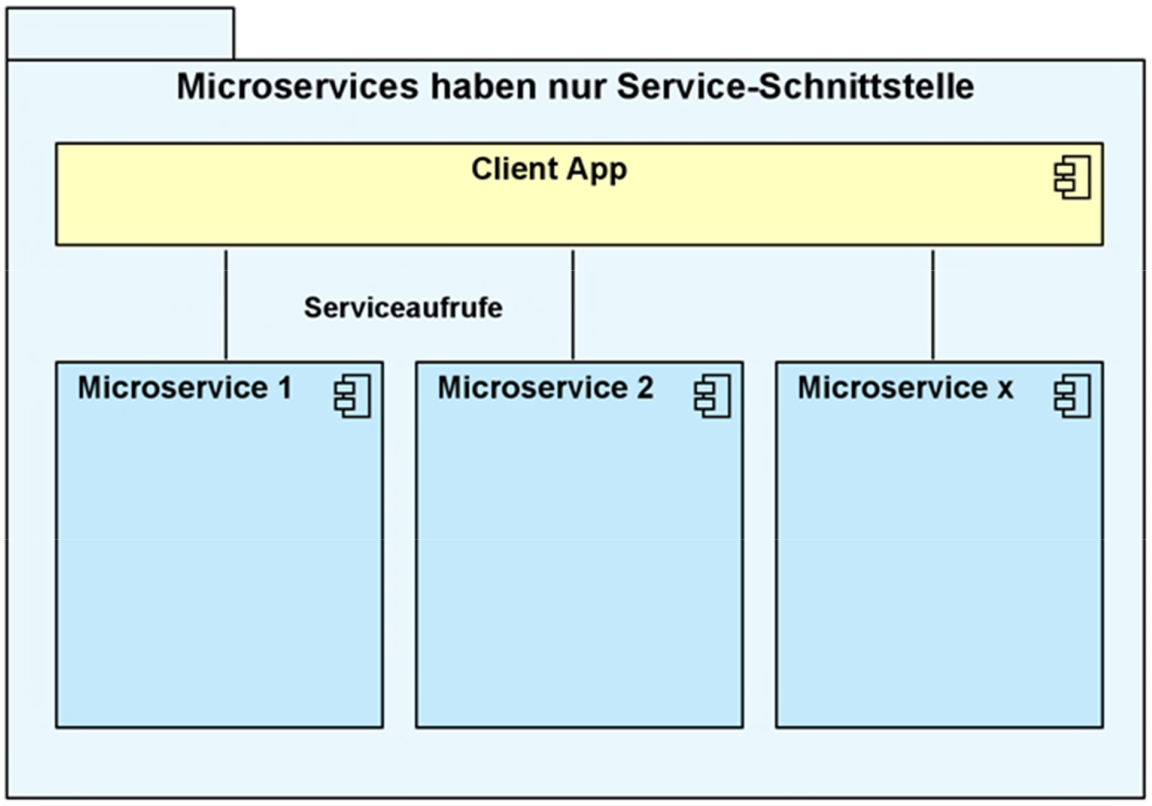
\includegraphics[width=0.8\linewidth]{microservices-ui-3.png} \\

\textcolor{blue}{Strukturierungsoptionen für das GUI}

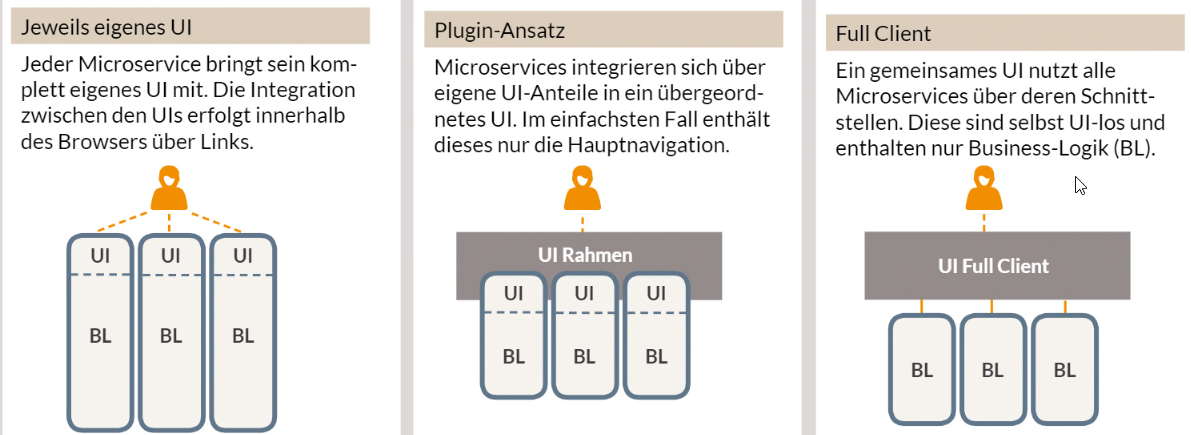
\includegraphics[width=\linewidth]{clients-gui-structures.png}


\vfill\null
\columnbreak

Beispiel

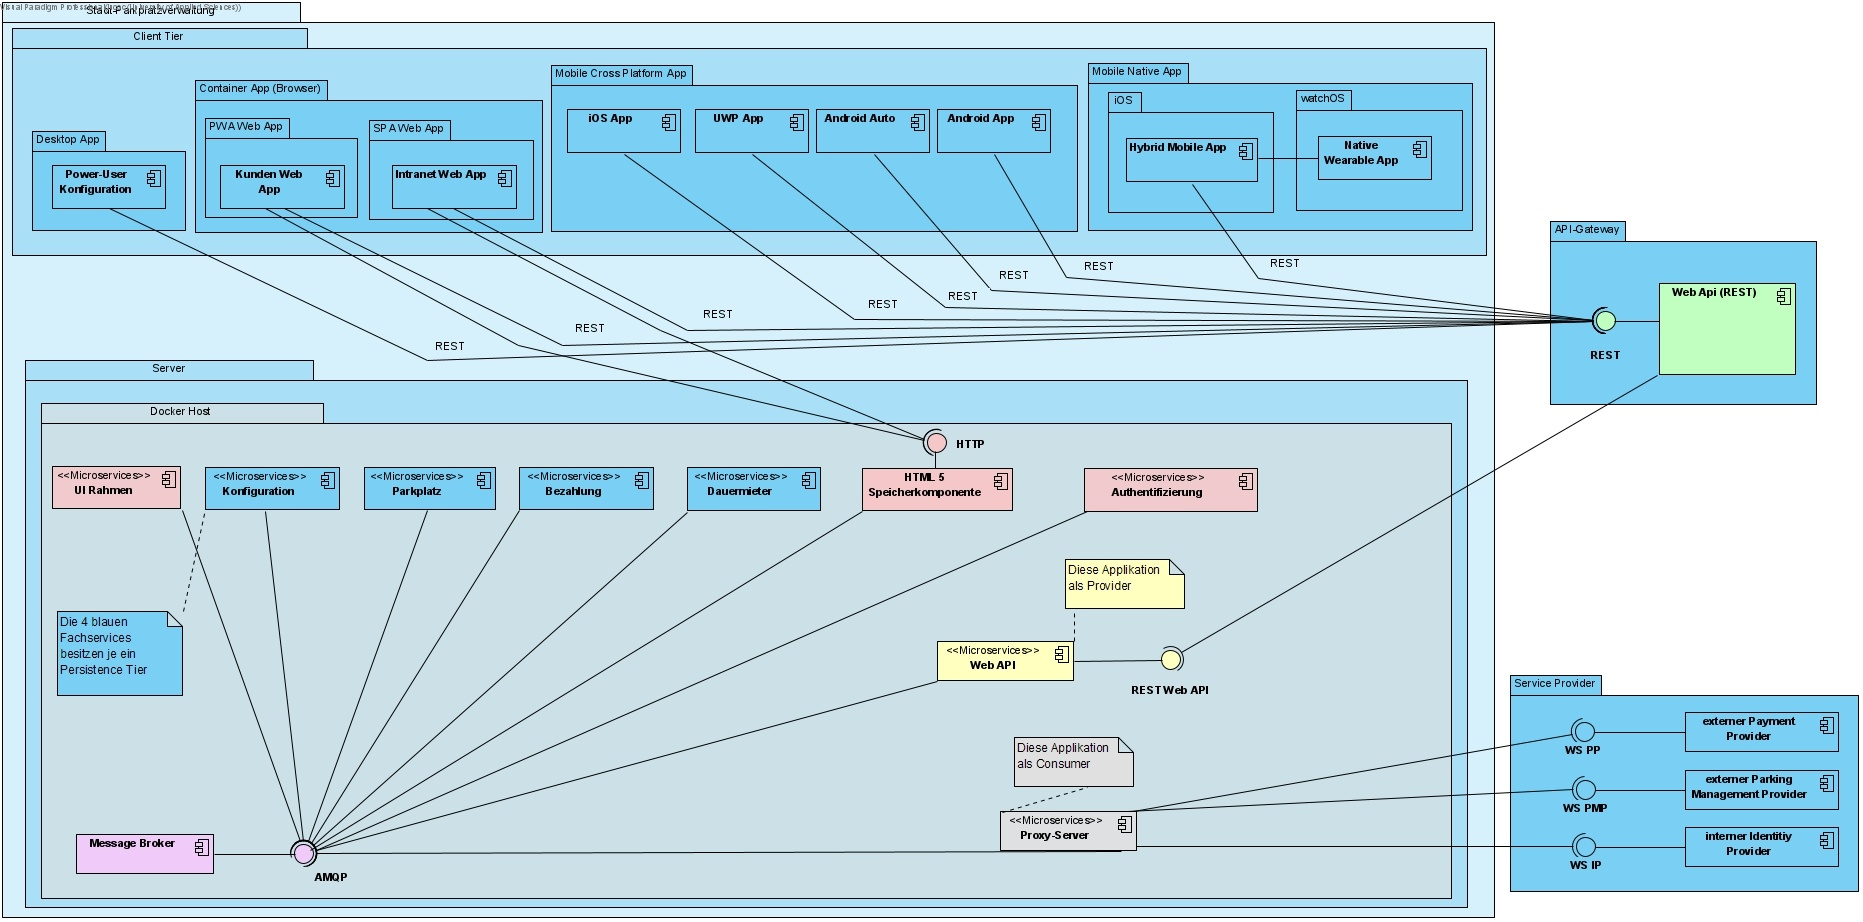
\includegraphics[width=2.1\linewidth]{clients-example-cars.png} \\

Full Client mit eigener Persistenz

eignet sich bei Angebot unterschiedlicher App-Arten

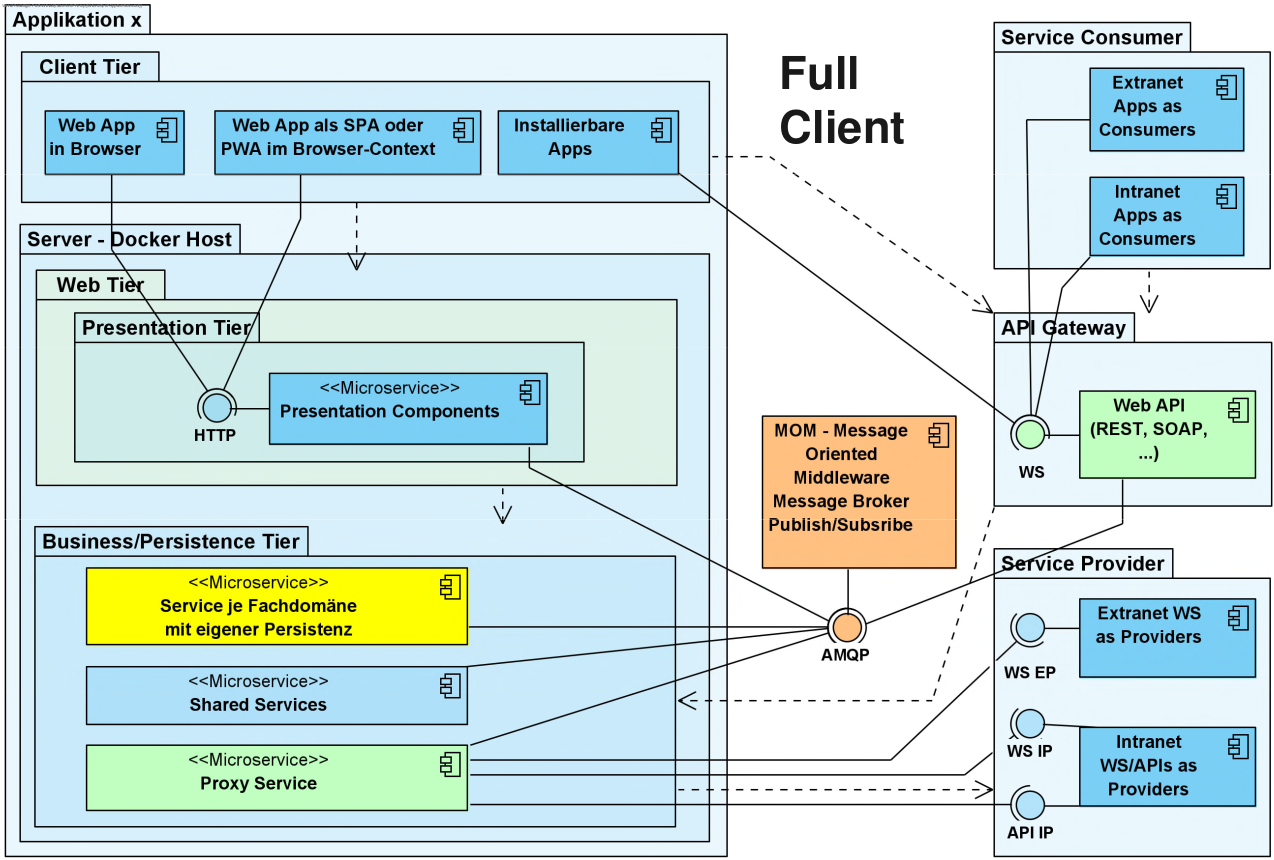
\includegraphics[width=\linewidth]{microservices-full-client.png}

Full Client mit separater Persistenz

Eignet sich bei der Migration einer bestehenden Mehrschichtenarchitektur in eine Microservice-Umgebung

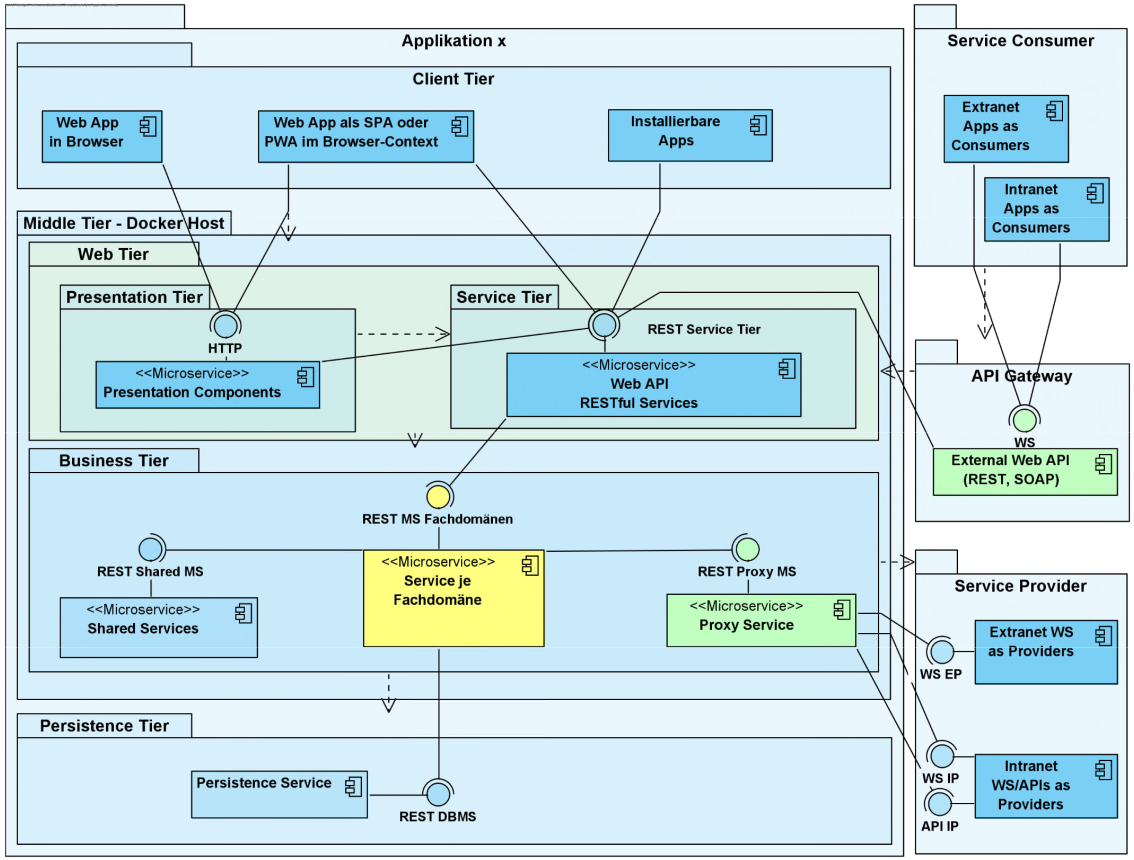
\includegraphics[width=\linewidth]{microservices-full-client-2.png}

\columnbreak

\vfill\null

\columnbreak

\subsubsection{Prüfungsfragen}

\begin{itemize}
    \item Was ist DaaS, aus welchen Komponenten besteht deren Infrastruktur und welche Vorteile ergeben sich für den Anwender sowie den Betreiber der IT? \\
    \textcolor{blue}{Device as a Service. Sind Virtuelle Desktops. Faster deployment and decommissioning of active end users. Reduced downtime for IT support. Cost savings. Increased Device flexibility, Enhanced Security}
    \item Wie funktioniert AJAX und welcher Nutzen ergibt sich für die UX? \\
    \textcolor{blue}{Seiten können dynamisch asynchron Nachgeladen werden.}
    \item Was ist der Unterschied zwischen AR und VR? \\
    \textcolor{blue}{AR verwendet real-world Settings und VR ist komplett virtuell}
    \item Welche drei Sprachen kommen in einer Web App primär zur Anwendung und welche Funktionen übernehmen diese? \\
    \textcolor{blue}{HTML, CSS und JavaScript}
\end{itemize}

        \vfill\null
        \columnbreak
        \subsection{Serverseitige Architektur}

\subsubsection{Skriptsprachen}

PHP, Python, Ruby, Node.js

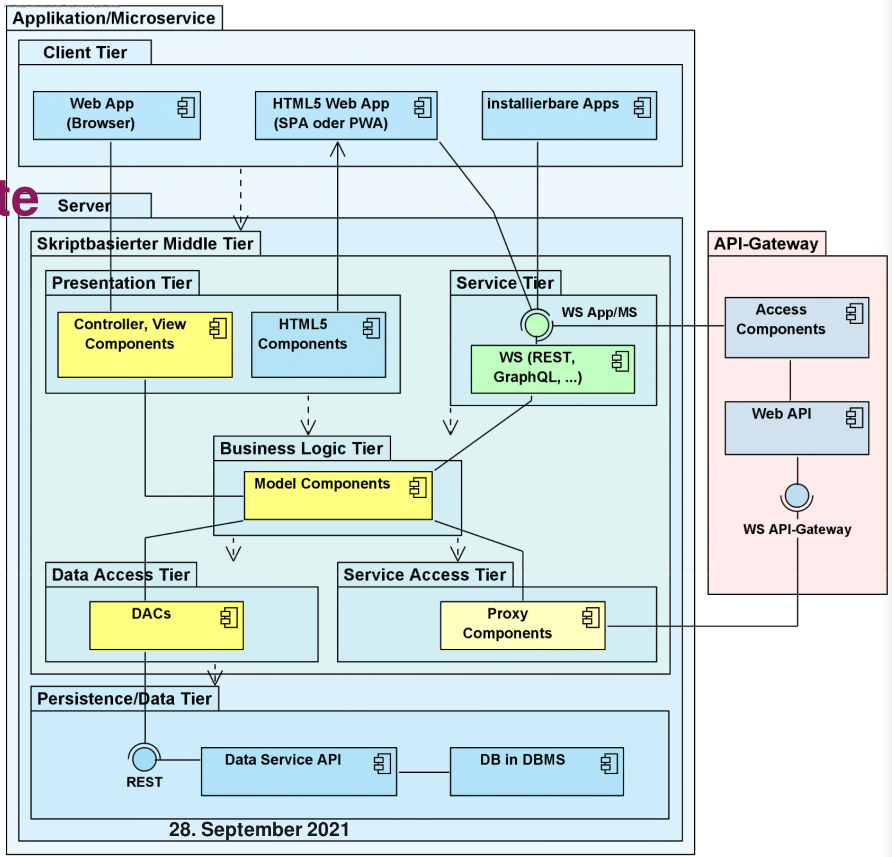
\includegraphics[width=\linewidth]{servers-reference-full-stack.png} \\

\subsubsection{node.js Architektur}

\includegraphics[width=\linewidth]{servers-nodejs.png} \\

\textbf{Mikroarchitektur}

eines Microservice

\includegraphics[width=\linewidth]{servers-example.png}

asynchrone Kommunikation, Cache-DB \\

\columnbreak
Beispiel

\includegraphics[width=\linewidth]{servers-nodejs-example.png}

\subsubsection{.NET Architektur}

\textbf{Merkmale}

Mehrere Programmiersprachen

\begin{itemize}
    \item \textcolor{blue}{C\#} C sharp, objektorientiert, ähnlich wie Java
    \item \textcolor{blue}{VB} Visual Basic
    \item \textcolor{blue}{F\#} funktionale Programmiersprache
\end{itemize}
\vspace{10pt}
Client-Tier

\begin{itemize}
    \item \textcolor{blue}{UX} User Experience
    \item \textcolor{blue}{UWP} Universal Windows App
    \item \textcolor{blue}{Xamarin} Multiplattform Mobile Apps
\end{itemize}
\vspace{10pt}
Web-Tier

realisiert mit IIS, Apache, NGINX und in-memory Kestrel

\includegraphics[width=\linewidth]{servers-dotnet-web-tier.png}

Web App

\begin{itemize}
    \item \textcolor{blue}{ASP.NET} Active Server Pages
\end{itemize}
\vspace{10pt}
Data Access

\begin{itemize}
    \item \textcolor{blue}{ORM} Obect-Relational Mapping, Entity Framework
    \item \textcolor{blue}{ODBC} Open Database Connectivity – direkt mit SQL!
    \item \textcolor{blue}{LINQ} Language Integrated Query
    \item \textcolor{blue}{ADO.NET} Active Data Object
\end{itemize}
\vspace{10pt}
\columnbreak
\textbf{Full Stack .NET}

\includegraphics[width=\linewidth]{servers-dotnet-reference.png}

\textbf{Mikroarchitektur}

\includegraphics[width=\linewidth]{servers-dotnet-micro.png}

\begin{itemize}
    \item Zugriff erfolgt über eine REST-Schnittstelle, die mit einer Azure Web-App entwickelt ist
    \item Fachlichen Funktionen sind als Azure Functions umgesetzt $\rightarrow$ diese kommunizieren asynchron über den Azure Service Bus
    \item dokumentorientierte Cosmos DB hält die Daten persistent
    \item Azure Logic Apps realisiert die Integration mit den Service Providern
\end{itemize}

\columnbreak
\subsubsection{Jakarta EE}

\textbf{Merkmale}

\begin{itemize}
    \item Open Source/Community – geführt von Eclipse
    \item Eine standardisierte Programmiersprache
    \item Web-/Application-Container übernehmen diverse Funktionalitäten/Dienste
    \item viele Anbieter von Web- und Applicationserver
    \item viele IDE's (Integrated Development Environments)
\end{itemize}
\vspace{10pt}
Presentation Layer mit Web App Framework

\begin{itemize}
    \item \textcolor{blue}{JSF} JavaServer Faces, mit EL (Expression Language), Zugriff auf Methoden des Backing Bean
    \item \textcolor{blue}{Backing Bean} Java Klasse, hat Zugriff auf EJBs
\end{itemize}
\vspace{10pt}
Zugriff auf Persistenz (DB)

\begin{itemize}
    \item \textcolor{blue}{JPA} Java Persistence API $\rightarrow$ ORM Object Relational Mapping
    \item \textcolor{blue}{Entity Beans} objektrelationale Abbildung der SQL-DB
    \item \textcolor{blue}{JDBC} Java Database Connectivity (direkt mit SQL)
\end{itemize}
\vspace{10pt}
Applikationsserver

\begin{itemize}
    \item Apache TomEE
    \item GlassFish
    \item Oracle WebLogic
    \item IBM WebSphere
    \item WildFly
\end{itemize}
\vspace{10pt}
JRMP – Java Remote Method Invocation Protocol

\begin{itemize}
    \item \textcolor{blue}{RMI} Remote Method Invocation
    \item \textcolor{blue}{IIOP} Internet Inter ORB [Object Request Broker] Protocol
\end{itemize}

\textbf{Frameworks}

\begin{itemize}
    \item Spring/Spring Boot
    \item Jakarta EE
    \item Hadoop
    \item Play
    \item Grails
    \item Quarkus
\end{itemize}

\columnbreak
\textbf{Container-Architektur}

%\includegraphics[width=\linewidth]{servers-container.png} \\
\includegraphics[width=\linewidth]{servers-java-container.png} \\

Client

\begin{itemize}
    \item Applet Container
    \item Application Client Container
\end{itemize}
\vspace{10pt}
Server

Web Container / Web API (Application Programming Interface)

\begin{itemize}
    \item Web Services (REST oder SOAP)
    \item Web Tier
    \item bildet Schnittstelle zum Client Tier bzw. zu den Service Consumer
\end{itemize}
\vspace{10pt}
EJB-Container (Enterprise Java Bean)

\begin{itemize}
    \item Business Tier
    \item hält Geschäftslogik
    \item gehostet in Application Server
    \item Funktionen für das Software Lifecycle Management
    \item Instanziierung, Kontrolle und Skalierung der EJBs (Enterprise Java Beans) $\rightarrow$ EJB sind auf dem Server ausführbare Klassen
    \item \textcolor{blue}{Session Beans (sync)} Stateful, Stateless, Singleton
    \item \textcolor{blue}{Message Driven Bean (async)} mittels JMS (Java Message Service)
\end{itemize}
\vspace{10pt}
\textbf{Makroarchitektur}

\includegraphics[width=0.8\linewidth]{servers-java-macro.png} \\

\columnbreak
\textbf{Mikro-/Referenzarchitektur}

\includegraphics[width=\linewidth]{servers-java-reference.png} \\

\textbf{Example}

\includegraphics[width=\linewidth]{servers-java-example.png} \\

\textbf{Cloud}

Grundbausteine in AWS

IaaS, PaaS/FaaS

\columnbreak
\subsubsection{IoT}
verbindet physische Objekte mit der virtuellen Welt. Intelligente Geräte und Maschinen sind dabei miteinander und mit dem Internet vernetzt. Sie erfassen relevante Informationen über ihre unmittelbare Umgebung, analysieren diese und verknüpfen sie.

\textbf{Cyberphysical (Smart) Things}

Ambient Intelligence

\includegraphics[width=\linewidth]{servers-iot-smart-thing.png}

Ein technisches Gerät, dessen Funktionalitäten und herausragende Eigenschaften sich aus dem vernetzten Zusammenspiel von rechnerischen und physischen Komponenten ergeben. Die CPS-Technologie zielt darauf ab, die für die nahtlose Integration von Cyber- und physischen Systemen erforderlichen Prozesse, Netzwerke und Technologien zu entwickeln

\begin{itemize}
    \item Intelligente Lampe
    \item Smarter Kühlschrank
    \item Smartes Fahrrad
    \item Produktionsmaschine
\end{itemize}
\vspace{10pt}
\textbf{Industrie 4.0}

Vernetzung auf Basis von Cyber-Physical System, intelligente Vernetzung von Maschinen und Abläufen in der Industrie mit Hilfe von Informations- und Kommunikationstechnologie

\textcolor{blue}{RAMI 4.0}
Referenzarchitekturmodell Industrie 4.0

\begin{itemize}
    \item grundlegende Architektur für Industrie 4.0 unter Verwendung eines ausgeklügelten Koordinatensystems
    \item explizite Berücksichtigung des Lebenszyklus von Assets oder Gegenständen im Produktionsumfeld (erlaubt auch immaterielle Objekte)
\end{itemize}

\includegraphics[width=\linewidth]{servers-iot-rami-1.png}

\includegraphics[width=0.5\linewidth]{servers-iot-rami-2.png} \\

\textcolor{blue}{IIRA}

Industrial Internet Reference Architecture

\includegraphics[width=\linewidth]{servers-iot-iira.png}

\begin{itemize}
    \item \textcolor{blue}{business viewpoint} stellt den Bezug zwischen den Belangen der Stakeholder und ihrer unternehmerischen Ziele, Werte und Absichten und dem IIS im Zusammenhang im geschäftlichen und regulatorischen Kontext dar. Diese Belange sind geschäftsorientiert und etwa für Entscheider, Produktmanager und System-Ingenieure von Belang.
    \item \textcolor{blue}{usage viewpoint} skizziert die erwartete Anwendung des Systems. Gewöhnlich wird dieser Sichtpunkt als eine Abfolge von Aktivitäten von menschlichen oder logischen Nutzern dargestellt, die so die angestrebte Funktionalität herstellen und die Fähigkeiten des Systems bereitstellen und ausführen.
    \item \textcolor{blue}{functional viewpoint} legt den Fokus auf die funktionalen Komponenten des IIS, ihre Beziehung zueinander, ihre Struktur, ihre Schnittstellen, ihr Zusammenwirken und den Bezug und die Interaktion des Systems mit externen Bestandteilen, die das Gesamtsystem unterstützen oder erweitern.
    \item \textcolor{blue}{implementation viewpoint} enthält die Techniken, die nötig sind, um die funktionalen Bestandteile zu implementieren, ihre Kommunikation zu ermöglichen und die Abläufe im Lebenszyklus sicherzustellen.
\end{itemize}
\vspace{10pt}
\columnbreak
\textbf{Referenzarchitektur}

\begin{itemize}
    \item \textcolor{blue}{Edge Tier} Bereich, in welchem die stationären oder mobilen IoT Devices verortet sind
    \item \textcolor{blue}{Platform Tier} Serverbereich, in welchem sich die Daten und Software zur IoT-Lösung befinden
    \item \textcolor{blue}{Enterprise Tier} beinhaltet alle operativen Fachanwendungen, wie z.B. ERP, CRM, PLM usw.
\end{itemize}

\includegraphics[width=\linewidth]{servers-iot-reference.png}

\begin{itemize}
    \item \textcolor{blue}{Edge Gateway} übernimmt Funktionen wie das Device Management, Security-Funktionen, Datenfilterung und Aggregation
    \item \textcolor{blue}{Platform Tier} lauft auf einem zentralen Server
    \item \textcolor{blue}{Data Transform} lädt aufbereitete Daten in das zentrale DBMS
    \item \textcolor{blue}{Dashboard} informiert berechtigte Stakeholder über aktuellen Stand
    \item \textcolor{blue}{Operationsmodul} enthält verschiedene Algorithmen zur Erzeugung von Seuerinformationen, welche zum Edge Gateway zurück fliessen
\end{itemize}
\vspace{10pt}
\textbf{Beispiele}

\includegraphics[width=\linewidth]{servers-iot-example.png}

\begin{itemize}
    \item Kunden verfügen über einen Smart Shelf
    \item Smart Goods sind mit IoT-Funktionalitäten ausgerüstet $\rightarrow$ Für den Unterhalt und die Einhaltung der Servicefenster während der Garantie sind diese mit dem Edge Gateway verbunden
    \item Edge Gateway tauscht Messages über MQTT mit AWS IoT Core aus
    \item AWS IoT Events nimmt Sensordaten entgegen und verarbeitet diese Referenzarchitektur
    \item Daten werden entweder in der DynamoDB gespeichert und/oder messages über den AWS
    Simple Queue Services Borker ausgetauscht
    \item Je nach Informationen löst der E-Shop Wartungshandlungen bzw. Bestellungen aus
\end{itemize}
\vspace{10pt}
\columnbreak
\textbf{Cloud}

\includegraphics[width=1.5\linewidth]{servers-iot-azure.png}

\includegraphics[width=1.5\linewidth]{servers-iot-aws.png}

\vfill\null
\columnbreak

\vfill\null
\columnbreak

\subsubsection{Prüfungsfragen}

\begin{itemize}
    \item Welche Funktion übt der Service Tier aus? Welche drei Spezifikationen stehen Ihnen in Jakarta EE dafür zur Verfügung? \\
    \textcolor{blue}{Für Datenaustausch mit den Client und Umsystemen. JAX-WS, JAX-RS und JAX-RPC}
    \item In welchem Szenario in Bezug auf die Funktionalität der Applikation macht ein Business Workflow Tier Sinn? \\
    \textcolor{blue}{Wenn Kunden applikationsinterne Workflows benötigen}
    \item Inwiefern erhöht die für den Anwender frei definierbaren Geschäftsregeln die Flexibilität des Einsatzes einer Applikation? Wo sind deren Grenzen? \\
    \textcolor{blue}{Antwort}
    \item Auf welchen Plattformen (OS) laufen .NET 5-Applikationen? \\
    \textcolor{blue}{Windows, macOS und Linux}
    \item Skizzieren Sie eine .NET Mehrschichtenarchitektur mit einer ASP.NET MVC Client-App, einem Zugriff auf einen Payment Service Provider so wie der Verwendung des MS SQL-Servers \\
    \textcolor{blue}{Antwort}
    \item Wie verorten Sie die drei Begriffe: J2EE, Jakarta EE, Java EE 8 zeitlich und inhaltlich? Welche Organisation stand bzw. steht jeweils dahinter? \\
    \textcolor{blue}{J2EE $\rightarrow$ Sun (1999-2003), Java EE 8 $\rightarrow$ Oracle (2017), Jakarta EE $\rightarrow$ Eclipse Foundation (2019)}
    \item Wie unterscheidet sich der Aufbau des Middle Tier in .NET gegenüber Jakarta EE? \\
    \textcolor{blue}{Siehe dessen Referenzarchitekturen}
    \item Beschreiben Sie die Stationen des Datenflusses ausgehend von Sensor-Daten in einem IoT Device, welche letztendlich dazu führen, dass das PLM (Product Lifecycle Management) neue Anweisungen für die Aktuatoren sendet \\
    \textcolor{blue}{Edge Gateway $\rightarrow$ Platform Gateway $\rightarrow$ Analytics Machine Learning AI $\rightarrow$ Domain Applications}
\end{itemize}

        \newpage
        \section{Anwendungsintegrationsarchitektur}
        
\textbf{Organisationsgrenzen}

\begin{itemize}
    \item \textcolor{blue}{Organisationsintern} Enterprise Architecture Integration (EAI)
    \item \textcolor{blue}{Organisationsübergreifend} B2x, B2B = Business to Business (Lieferanten, Logistikpartner, Finanzinstitute), B2C = Business to Consumer, B2A = Business to Administration (Behörden, Steuerämter, Zoll), E-Business: \\
    \includegraphics[width=\linewidth]{integration-e-business.png}
\end{itemize}
\vspace{10pt}
\textbf{MSP (Managed Service Provider)}

Cloud Service Intermediäre, der Vorteil für den Kunden ist, dass er technisch nur eine Schnittstelle unterhalten muss. Über Adresse und Wahl des Messagetyps werden Geschäftspartner angesteuert

\begin{itemize}
    \item \textcolor{blue}{Identity SP} Identity Broker, Self-Service, Passwort Management, Single-Sign-on (SSO), Identity und Access Governance \\ $\rightarrow$ Facebook, Google, auth0
    \item \textcolor{blue}{EDI SP} Integration mit EDICFACT, ebXML, CXML, xRechnung usw. \\ $\rightarrow$ Mulesoft, SAP Ariba, Seeburger
    \item \textcolor{blue}{Message SP} einheitliche Schnittstelle für E-Mail, SMS, MMS, WhatsApp, RCS (Rich Communication Services) und Sprachnachrichten \\ $\rightarrow$ - twilio, MessageBird
    \item \textcolor{blue}{Payment SP} Einheitliche Schnittstelle für Zahlungsinstitute, Kreditkarten, Debitkarten, weitere elektronische Zahlungsmittel \\ $\rightarrow$ Payrexx, Stripe
    \item \textcolor{blue}{Karten/Geodaten SP} Landkartendienst \\ $\rightarrow$ Google Maps
    \item \textcolor{blue}{Daten SP} Datendienst wie Adress-, Markt-, Statistik-Daten \\ $\rightarrow$ Finanzinformationen von Six-Group, Open Data Swiss
\end{itemize}

        \vfill\null
        \columnbreak
        
\subsection{Integration auf Präsentationsebene}

für Client-Tier

\subsubsection{Client-App-orientierte Integration}

Von unterschiedlichen Anwendungen in eine einheitliche Client-Oberfläche. Integration der EC-Karte und Checkout über Payment Provider. Vorteil ist die rasche Realisierung mit Widgets. Nachteil sind die Abhängigkeiten

\begin{itemize}
    \item UI-Rahmen App
    \item Widgets
    \item Identity-Provider für Login
    \item Payment-Provider für Zahlungsprozess
\end{itemize}

\subsubsection{Portalorientierte Integration}
thematisch ausgerichtete Portallösung. Bsp. Mitarbeiterportal. Primär ein SSO (Single Sign-on). Vorteil Stakeholder muss nur einen Zugangslink mit Zugangsinformationen merken.

\begin{itemize}
    \item Lieferantenportal
    \item Kundenportal
    \item Mitarbeiterportal
\end{itemize}

\includegraphics[width=\linewidth]{integration-presentation-portal.png}

\subsubsection{Geschäftsprozessorientierte Integration}

mittels WfMS (Workflow Management System). Vorteil Hohes Einsparungspotenzial bei stark strukturierten, komplexen und häufig ausgeführten Workflows

\begin{itemize}
    \item Funktion einer Middleware
    \item Integriert in einer Fachapplikation
    \item dedizierten WfMS
\end{itemize}
\vspace{10pt}
\textbf{WfMC Referenzmodell}

\includegraphics[width=\linewidth]{integration-wfmc-workflow.png} \\

\textcolor{blue}{Process Definition}

GP-Prozessmodellierung mit BPMN (Business Process Modeling and Notation)

\includegraphics[width=\linewidth]{integration-omg-bpmn.png}

Funktionsübersicht

\includegraphics[width=\linewidth]{integration-omg-functions.png} \\

\textbf{WfMS Referenzarchitektur}

\includegraphics[width=\linewidth]{integration-wfms-workflow.png}


        \vfill\null
        \columnbreak
        \subsection{Integration auf Applikationsebene}
für Middle-Tier

Punkt-zu-Punkt-Integrationen führt zur Verwaltung von x Schnittstellen

\begin{itemize}
    \item API, EAI, B2x
    \item Service-Oriented Architecture (SOA) ist eine Voraussetzung
    \item \textcolor{blue}{Technische Heterogenität} der Plattformen unterschiedlicher Systeme überwinden und auch Legacy Systeme miteinbeziehen
    \item Cloud-Services und Social Media Services integrieren
    \item Begrifflichkeiten und Schwerpunkte der Fachdomänen berücksichtigen und Übersetzungslayer vorsehen
    \item Schnittstellen mit Spezifikationen und Mapping-Informationen verwalten
    \item Integrations-Middleware auswählen
    \item Wahl der Transportprotokolle, sowie Message-Normen
\end{itemize}
\vspace{10pt}

\subsubsection{Schnittstellen}

\includegraphics[width=\linewidth]{integration-contract.png} \\

\textbf{Adapter}

\includegraphics[width=\linewidth]{integration-adapter.png} \\

\begin{itemize}
    \item \textcolor{blue}{API} Application Programming Interface, Port (Adressierung)
    \item \textcolor{blue}{Adapter (Konnektor)} enthält alle Spezifika einer Schnittstelle, fungiert als Proxy (Stellvertreter)
\end{itemize}
\vspace{10pt}
\textbf{Gateway}

\includegraphics[width=\linewidth]{integration-gateway.png} \\

\columnbreak
\textbf{Wrapper}

\includegraphics[width=\linewidth]{integration-wrapper.png} \\

\textbf{Integration Middleware (IM)}

bietet zwischen organisationsinternen und externen Applikationen einen workflowgetriebenen automatischen Datenaustausch (Integration-Broker).

bildet die Datendrehscheibe der Organisation, sie bietet die passenden APIs für alle internen Apps, wie Fach- und Querschnittsapplikationen an \\

\textcolor{blue}{APIs für...}

\begin{itemize}
    \item Kommunikationsdienst
    \item Transformationsdienst
    \item Datenroutingdienst
    \item Workflowdienst
    \item Monitoringdienst
\end{itemize}
\vspace{10pt}
\textcolor{blue}{Funktionen}

\begin{itemize}
    \item Connectivity zu Umsystemen über Standard-Konnektoren
    \item Synchrone Echtzeitverarbeitung mittels API-Gateway
    \item Asynchrones Messaging über Message-Broker
    \item Messagekonversion mittels Datenmapping und Codekonversionen
    \item Modellierung von Integrations-Workflows
\end{itemize}

\subsubsection{Integrationsarchitekturentwurf (Modellierung)}

Beschreibung einer Applikationsschnittstelle (Notation)

\includegraphics[width=\linewidth]{integration-draft-arch.png}

\begin{itemize}
    \item Komponente $\rightarrow$ ganze Applikation. Kann als Consumer oder Provider agieren
    \item Provider App bietet APIs an
    \item API ist mit dem höchsten Protokoll angeschrieben. Wichtigsten Varianten in der Notiz ersichtlich
    \item Consumer App hat Assoziation mit halboffenem Kreis. Beschriftung zu Semantik, Struktur und Codierung
    \item Client-App ist nur dann zu modellieren, wenn diese nicht Teil einer Gesamtapplikation ist
    \item Realtime-Verbindungen verwenden Fachapplikationen direkt
    \item EDI Integrationen sind meist via Integration Middleware zum EDI Service Provider verbunden
    \item Asynchrone Integration erfolgt über Message Broker (MOM)
\end{itemize}

\subsubsection{Referenz Integrationarchitektur}

Wichtig: eine Applikationskomponente enthält alle Schichten (d.h. Client und Server-
Komponenten)!

\includegraphics[width=\linewidth]{integration-reference-architecture.png} \\

\textbf{Beispiel}

\includegraphics[width=\linewidth]{integration-example.png}

\begin{itemize}
    \item E-Shop sendet E-Mails über SMTP-Schnittstelle des Exchange-Mailservers
    \item Als alternatives Login können die Kunden Google als Identity Provider verwenden
    \item Zahlungsabwicklung läuft über BS-PAYONE
    \item Periodischer Datenaustausch mit internen Systemen, wie ERP und CRM erfolgt über eine REST-Schnittstelle
    \item cXML-Messages mit den Kunden über Integration Middleware zur SOAP-Schnittstelle des EDI Service Providers.
    \item WhatsApp und SMS gehen über Mulesoft zum Message Service Provider
\end{itemize}


        \vfill\null
        \columnbreak
        \subsection{Integration auf Datenebene}

für Data/Persistence Tier

\subsubsection{Gemeinsame Datenbank}

Zugriff meist über REST, GraphQL oder über das Extranet mit OData zwecks operativer aktueller Nutzung

\includegraphics[width=\linewidth]{integration-datebase-shared.png}

\subsubsection{Zentrale, historisch orientierte Datenhaltung}

Zentrales Data Warehouse bzw. Data Lake zwecks Analyse

\includegraphics[width=\linewidth]{integration-datebase-central.png}

\begin{itemize}
    \item \textcolor{blue}{Data Warehouse} zentrales Datenmodell mit strukturierten Daten
    \item \textcolor{blue}{Data Lake} wenig / nicht strukturiert und meist 1:1 Quelldaten
    \item \textcolor{blue}{Data Marts} themenspezifische Auszüge aus Data Warehouse
\end{itemize}
\vspace{10pt}
\textbf{Aufbereitung der Daten für den Load}

\begin{itemize}
    \item \textcolor{blue}{Feldtransformation} Adressdaten sauber auseinander nehmen
    \item \textcolor{blue}{Codetransformation} einheitliche Codes im Data Warehouse
    \item \textcolor{blue}{Aggregation} nicht notwendige Detailtransaktionen
    \item \textcolor{blue}{Data-Enrichment} Adresse mit externen Marktinformationen anreichern
    \item \textcolor{blue}{Data-Cleansing} Daten überprüfen und bereinigen
\end{itemize}

\vfill\null
\columnbreak

\subsubsection{Prüfungsfragen}

\begin{itemize}
    \item Welches sind die in diesem Kapitel angesprochenen zwei Integrationsdimensionen? \\
    \textcolor{blue}{Organisationsinterne und organisationsübergreifende Integration}
    \item Auf welchen drei Ebenen kann die IT-Integration stattfinden? Auf welche Schichten
    des Mehrschichtenmodells beziehen sich diese? \\
    \textcolor{blue}{Präsentationsebene (Client Tier), Applikationsebene (Middle Tier) und Datenebene (Data / Persistence Tier)}
    \item Welche drei Varianten stehen bei der präsentationsorientierten
    Integration zur Verfügung? Nennen Sie zu jeder Variante je einen Vorteil \\
    \textcolor{blue}{Client-App-orientierte Integration, Portalorientierte Integration, Geschäftsprozessorientierte Integration}
    \item Welche wichtigen Funktionen übernimmt eine Integration Middleware (IM)? Geben Sie mindestens vier gebräuchliche synonyme Begriffe zu IM \\
    \textcolor{blue}{Integration Bus, Enterprise Service Bus, Integration Broker oder Hub}
    \item Zeichnen Sie mit dem UML-Komponentendiagramm gemäss den Vorgaben in diesem Kapitel die folgende Situation: ein ERP-System konsumiert den SOAP EDI-Service eines EDI-Service Providers und setzt dabei ebXML ein \\
    \textcolor{red}{Keine}
    \item Legen Sie den Unterschied zwischen einem Data Warehouse und einem Data Lake in 2-3 ganzen Sätzen dar \\
    \textcolor{blue}{Data Warehouse ist ein zentrales Datenmodell mit strukturierten Daten. Ein Data Lake hingegen hat wenig bis nicht strukturierte Daten, welche meist Quelldaten sind.}
    \item Über welche Schritte gelangen die Daten von einem ERP bis zu einer BI-Applikation? Geben Sie zu jedem Schritt eine kurze Erläuterung \\
    \textcolor{blue}{ETL (Extraction, Transformation, Load) $\rightarrow$ Data Store (Data Warehouse oder Data Lake) $\rightarrow$ BI Applikation}
\end{itemize}



    \end{multicols*}

    \begin{multicols*}{2}
        \setlength{\columnseprule}{0.4pt}

        \includegraphics[width=0.7\linewidth]{example-1.png}

        \includegraphics[width=\linewidth]{example-2.png}

        \includegraphics[width=\linewidth]{example-3.png}

        \includegraphics[width=\linewidth]{example-4.png}

        \includegraphics[width=\linewidth]{soa-example.png}

        \includegraphics[width=\linewidth]{integration-omg-bpmn.png}
    \end{multicols*}

\end{document}
